\documentclass[conference]{IEEEtran}
%\IEEEoverridecommandlockouts
% The preceding line is only needed to identify funding in the first footnote. If that is unneeded, please comment it out.

\usepackage{mathtools}  % for special symbols such as :=
\usepackage{xspace}
\usepackage{achinDefs}


\usepackage{tikz}
\usepackage[utf8]{inputenc}
\usepackage{pgfplots} 
\usepackage{pgfgantt}
\usepackage{pdflscape}
\pgfplotsset{compat=newest} 
\pgfplotsset{plot coordinates/math parser=false}
\newlength\fwidth
\newlength\hwidth

%%%%%%%%%%%%%%%%% Macros used in the paper %%%%%%%%%%%%%%%%%%%%

\newtheorem{definition}{Definition}

% Auto-regressive vector
\newcommand{\arvec}[1]{\ensuremath{\boldsymbol{#1}}}  % ^{\leftarrow}
\def\Pbatt{\ensuremath{b}}
\def\Ptotal{\ensuremath{p}}
\def\Pbmax{\ensuremath{\Pbatt_{\mathrm{max}}}}
\def\Pbmin{\ensuremath{\Pbatt_{\mathrm{min}}}}
\def\SOCmax{\ensuremath{s_{\mathrm{max}}}}
\def\SOCmin{\ensuremath{s_{\mathrm{min}}}}

\newcommand{\GaussianDist}[2]{\ensuremath{\operatorname*{\mathcal{N}}\left(#1, #2\right)}}  % Gaussian distribution given mean and variance
\newcommand{\GaussianDistSmall}[2]{\ensuremath{\operatorname*{\mathcal{N}}(#1, #2)}}  % Gaussian distribution given mean and variance

% Typeset predicted variables. Usage:
% \predict{k}{u} --> predicted u at k | t
% \predict[\tau]{k}{u} --> predicted u at k | \tau
\newcommand{\predict}[3][t]{\ensuremath{#3}_{#2 | #1}}

\newcommand{\sigmamax}[1][0]{\ensuremath{\overbar{\sigma}_{#1}}}

\newcommand{\eg}{e.g.,\xspace}
\newcommand{\ie}{i.e.,\xspace}
\newcommand{\etc}{etc.\xspace}
\newcommand{\cf}{cf.~}

% Some commonly used math functions/operators
\DeclareMathOperator*{\argmin}{arg\,min}
\DeclareMathOperator*{\argmax}{arg\,max}
\DeclareMathOperator*{\minimize}{minimize}
\DeclareMathOperator*{\maximize}{maximize}
\DeclareMathOperator{\sgn}{sgn}  % the signum/sign function

\newcommand{\RR}{\mathbb{R}\xspace}  % Real set
\newcommand{\NN}{\mathbb{N}\xspace}  % Natural number set
\newcommand{\QQ}{\mathbb{Q}\xspace}  % Rational number set
\newcommand{\CC}{\mathbb{C}\xspace}  % Complex number set
\newcommand{\ZZ}{\mathbb{Z}\xspace}  % Integer number set
\newcommand{\EE}{\mathbb{E}\xspace}  % Expectation
\newcommand{\PP}{\mathbb{P}\xspace}  % Probability
\newcommand{\BB}{\mathbb{B}\xspace}  % Logic set {true, false}

% some fixes
%\linespread{0.915}
%\setlength{\textfloatsep}{4pt}


% make algo small
%\makeatletter
%\renewcommand{\ALG@beginalgorithmic}{\small}
%\makeatother

\begin{document}

\title{Learning and Control using Gaussian Processes \\
	\vspace{0.1cm}
	\Large \textbf{Towards bridging machine learning and controls for physical systems}}


\author{\IEEEauthorblockN{Achin Jain$^{\star,\S}$, Truong X. Nghiem$^{\star,\S,\ddag}$, Manfred Morari$^{\S}$, Rahul Mangharam$^{\S}$}
\IEEEauthorblockA{\textit{$^{\S}$University of Pennsylvania, Philadelphia, PA 19104, USA} \\
\textit{$^{\ddag}$Northern Arizona University, Flagstaff, AZ 86011, USA} \\
$^{\star}$\textit{equal contribution}}
%\and
%\IEEEauthorblockN{2\textsuperscript{nd} Given Name Surname}
%\IEEEauthorblockA{\textit{dept. name of organization (of Aff.)} \\
%\textit{name of organization (of Aff.)}\\
%City, Country \\
%email address}
%\and
%\IEEEauthorblockN{3\textsuperscript{rd} Given Name Surname}
%\IEEEauthorblockA{\textit{dept. name of organization (of Aff.)} \\
%\textit{name of organization (of Aff.)}\\
%City, Country \\
%email address}
%\and
%\IEEEauthorblockN{4\textsuperscript{th} Given Name Surname}
%\IEEEauthorblockA{\textit{dept. name of organization (of Aff.)} \\
%\textit{name of organization (of Aff.)}\\
%City, Country \\
%email address}
}

\maketitle

%% ABSTRACT
\begin{abstract}
  Building physics-based models of complex physical systems like buildings and chemical plants is extremely cost and time prohibitive for applications such as real-time optimal control, production planning and supply chain logistics.  Machine learning algorithms can reduce this cost and time complexity, and are, consequently, more scalable for large-scale physical systems. However, there are many practical challenges that must be addressed before employing machine learning for closed-loop control. This paper proposes the use of Gaussian Processes (GP) for learning control-oriented models. We develop methods for the optimal experiment design of functional tests to learn models of a physical system, subject to stringent operational constraints and limited availability of the system.  Using a Bayesian approach with GP, our methods seek to select the most informative data for optimally updating an existing model.  We also show that black-box GP models can be used for receding horizon optimal control with probabilistic guarantees on constraint satisfaction through chance constraints. % of a real building for power demand curtailment in context of Demand Response.
  We further propose an online method for continously improving the GP model in closed loop with a real-time controller.
  Our methods are demonstrated and validated in a case study of building energy control and Demand Response.
\end{abstract}
%%% Local Variables:
%%% mode: latex
%%% TeX-master: "main"
%%% End:


\begin{IEEEkeywords}
Machine learning, Gaussian Processes, optimal experiment design, receding horizon control, active learning
\end{IEEEkeywords}

%% SECTIONS
\section{Introduction}

\todo[inline]{shorten and rephrase the CDC part}
\todo[inline]{Need a discussion on related work, including RT papers, GP papers \protect\cite{nghiemetal16gp}, especially for buildings.}

Machine learning and control theory are two foundational but disjoint communities. Machine learning requires data to produce models, and control systems require models to provide stability, safety or other performance guarantees. Machine learning is widely used for regression or classification, but thus far data-driven models have not been suitable for closed-loop control of physical plants. The challenge now, with using data-driven approaches, is to close the loop for real-time control and decision making.

Consider a multivariable dynamical system subject to external disturbances. The first and foremost requirement for making any decision is to obtain the underlying control-oriented predictive model of the system. With a reasonable forecast of the external disturbances, these models should predict the state of the system in the future and thus a predictive controller based on Model Predictive Control (MPC) can act preemptively to provide a desired behavior. In particular, MPC has been proven to be very powerful for multivariable systems in the presence of input and output constraints, and forecast of the disturbances. The caveat is that MPC requires a reasonably accurate physical representation of the system. This makes MPC unsuitable for control of complex plants such as natural gas processing, oil refineries, boilers, manufacturing plants, and buildings where the user expertise, time, and associated sensor costs required to develop a model are very high \cite{Sturzenegger2016,vzavcekova2014}.

There are two main reasons for model complexity. 
(1) The prime contributor is the change in model properties over time. Even if the model is identified once via an expensive route, as the model changes with time, the system identification must be repeated to update the model. Thus, model adaptability or adaptive control is desirable for such systems. 
(2) A secondary reason is the model heterogeneity which further prohibits the use of model-based control. For example, unlike the automobile or the aircraft industry, each building is designed and used in a different way. Therefore, this modeling process must be repeated for every new building. 
Due to aforementioned reasons, the control strategies in such systems are often limited to fuzzy logic rules that are based on best practices. 

The question now is, can we employ data-driven techniques to reduce the cost of modeling, and still exploit the benefits that MPC has to offer? We therefore look for automatic and data-driven approaches to control that are also adaptive, scalable and interpretable. We solve this problem with \textit{Data Predictive Control (DPC)} by bridging the gap between Machine Learning and Predictive Control.

\subsection{Challenges in bridging machine learning and controls}
\label{SS:practical_challenges}

The central idea behind DPC is to obtain control-oriented models using machine learning or black-box modeling, and formulate the control problem in a way that receding horizon control (RHC) can still be applied and the optimization problem can be solved efficiently.

It is important to note that the standard machine learning regression used for prediction is fundamentally different from using machine learning for control synthesis. In the former, all the inputs to the model (also called regressors or features) are known, while in the latter some of the inputs that are the control variables must be optimized in real-time for desired performance. 

We next discuss the practical challenges in using machine learning algorithms for control.

\noindent \textbf{(1) Data quality:} Most of the historical data that is available from complex systems like buildings are based on some rule-based controllers. Therefore, the data may not be sufficient to explain the relationship between the inputs and the outputs. To obtain richer data with enough excitation in the inputs, new experiments must be done either by sampling the inputs randomly or by a procedure for optimal experiment design (OED) \cite{Emery1998,Fedorov2010}. This paper proposes the use of GP i.e.~the estimate of variance in GP predictions to recommend control strategies for OED.

\noindent \textbf{(2) Computational complexity:} Depending upon the learning algorithm, the output from a learned model is a non-linear, non-convex and sometimes non-differentiable (eg.~Random Forests \cite{Friedman2001}) function of the inputs with no closed-form expression. Using such models for control synthesis where some of the inputs must be optimized can lead to computationally intractable optimization. Our previous work on DPC uses an adaptation of Random Forests which overcomes this problem by separation of variables to derive a linearized input-output mapping at each time step \cite{JainACC2017,JainCDC2017}.
This paper uses Gaussian Processes (GP) where the output mean and variance are analytical functions of the inputs, albeit non-convex.

\noindent \textbf{(3) Performance guarantees and robustness:} A desired characteristic for closed-loop control is to provide performance guarantees. This becomes hard when a black-box is used to replace a physical model. However, it is possible to provide probabilistic guarantees with a learning algorithm based on Gaussian Processes. DPC based on Gaussian Processes allows us to define chance constraints or account for model uncertainty in the cost while solving the optimization problem. This helps bound the performance errors with high confidence. Handling disturbance uncertainties or robustness to sensor failures in the DPC framework is part of our on-going work and is thus excluded from this paper.

\noindent \textbf{(4) Model adaptability:} It is often the case that the model properties change with time, and thus, the learned model must also be updated when required. The traditional mode of system identification, done repeatedly, can be time and cost prohibitive. In this paper, we discuss the active learning for GP models that allows to update the model from one season to another.

%\noindent \textbf{(5) Interpretability of control decisions:} Besides the accuracy of synthesizing control strategies with machine learning in the loop, we are also interested in solutions that are interpretable and trustworthy. Thus, the DPC recommendations should have traceability so they can be verified to be stable and safe. This direction of research also forms part of our on-going work.

\subsection{Overcoming practical challenges}
To address these challenges, we can take two different approaches based on what level machine learning is used to learn the models.

\noindent \textbf{(1) Mix of black-box and physics-based models:} Here, we use machine learning only to learn the dynamics of a sub-system or to model uncertainties in the dynamics. An example of former is in the use of machine learning for perception and model-based control for low-level control in self-driving cars \cite{Urmson2008}. Examples on learn uncertainties in the models include \cite{Berkenkamp2015,Desaraju2016}.

\noindent \textbf{(2) Fully black-box models:} The full dynamical model can also be obtained using only machine learning algorithms. This deviates from the traditional notion of system identification where a physics-based structure is assumed to begin with. An example would be fully autonomous control using camera vision where control actions are mapped to raw image pixels \cite{Bojarski2016}. The catch here is that, prior to learning, sufficiently large data could be generated by running the car in simulations.

For the application to building control in context of Demand Response, where there is a massive cost to physical modeling, this paper explores the latter route to bypass the modeling difficulties as summarized in \cite{Sturzenegger2016}. The model-free approach allows to scale this methodology to multi-building campus and in general to any more applications like control of autonomous systems.

\begin{figure}[!t]
	\centering
	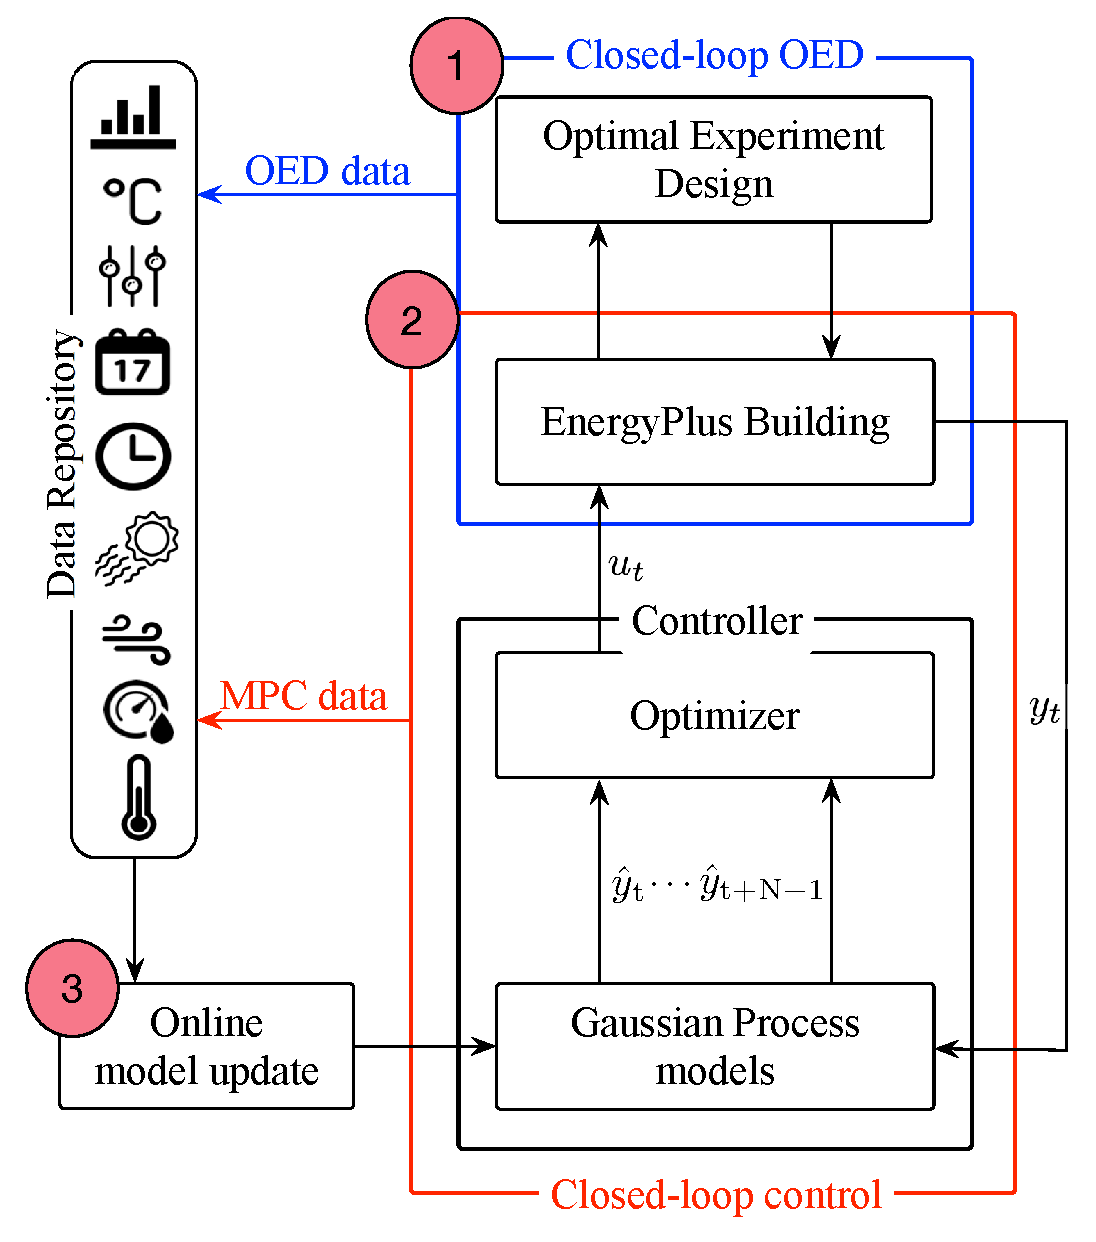
\includegraphics[width=1\linewidth]{figures/overview.eps}
	\caption{Paper organization and contributions}
	\captionsetup{justification=centering}
	\label{F:intro}
\end{figure}

\subsection{Contributions}

\todo[inline]{revisit when OED and CONTROL sections are ready}

This paper has the following contributions:
\begin{enumerate}
	\item Optimal experiment design for recommending control strategies for functional test
	\item MPC using Gaussian Processes for real-time control
	\item Active learning with a MPC in closed-loop
\end{enumerate}



%%% Local Variables:
%%% mode: latex
%%% TeX-master: "main"
%%% End:

\section{Gaussian Processes}
\label{S:gp}

In this section, we briefly introduce modeling with Gaussian Process (GP) and its applications in control.
More details can be found in \cite{Rasmussen2006} %on GP for machine learning and in
and \cite{Kocijan2016}. % on GP modeling of dynamic systems.

\begin{definition}[\cite{Rasmussen2006}]
A Gaussian Process is a collection of random variables, any finite number of which have a joint Gaussian distribution.
\end{definition}
Consider noisy observations \(y\) of an underlying function \(f: \RR^n \mapsto \RR\) through a Gaussian noise model: \(y = f(x) + \GaussianDist{0}{\sigma_n^2}\), \(x \in \RR^n\).
A GP of \(y\) is fully specified by its mean function \(\mu(x)\) and covariance function \(k(x,x')\),
\begin{align}
\label{E:gp:prior}
\mu(x; \theta) &= \EE [f(x)] \\
k(x,x'; \theta) &= \EE [(f(x)\!-\!\mu(x)) (f(x') \!-\! \mu(x'))] + \sigma_n^2 \delta(x,x') \nonumber
\end{align}
where \(\delta(x,x')\) is the Kronecker delta function.
The hyperparameter vector \(\theta\) parameterizes the mean and covariance functions.
This GP is denoted by \(y \sim \mathcal{GP}(\mu, k; \theta)\).

Given the regression vectors \(X = [x_1, \dots, x_N]^T\) and the corresponding observed outputs \(Y = [y_1, \dots, y_N]^T\), we define training data by $\D = (X, Y)$. The distribution of the output \(y_\star\) corresponding to a new input vector \(x_\star\) is a Gaussian distribution \(\GaussianDist{\bar{y}_\star}{\sigma_\star^2}\), with mean and variance given by
\begin{subequations}
\label{E:gp-regression}
\begin{align}
\bar{y}_\star &= g_{\mathrm{m}} (x_{\star}) \coloneqq \mu(x_\star) + K_\star K^{-1} (Y - \mu(X))\\
\sigma_\star^2 &= g_{\mathrm{v}} (x_{\star}) \coloneqq K_{\star \star} - K_\star K^{-1} K_\star^T \text,
\end{align}
\end{subequations}
where \(K_\star = [k(x_\star, x_1), \dots, k(x_\star, x_N)]\), \(K_{\star \star} = k(x_\star, x_\star)\), and $K$ is the covariance matrix with elements \(K_{ij} = k(x_i, x_j)\).

Note that the mean and covariance functions are parameterized by the hyperparameters $\theta$, which can be learned by maximizing the likelihood: \(\argmax_\theta \Pr(Y \vert X, \theta)\).
The covariance function \(k(x,x')\) indicates how correlated the outputs are at \(x\) and \(x'\), with the intuition that the output at an input is influenced more by the outputs of nearby inputs in the training data $\D$.
In other words, a GP model specifies the structure of the covariance matrix of, or the relationship between, the input variables rather than a fixed structural input--output relationship.
It is therefore highly flexible and can capture complex behavior with fewer parameters.
An example of GP prior and posterior is shown in Fig.~\ref{F:gp:prior:posterior}. We use a constant mean function and a combination of squared exponential kernel and rational quadratic kernel as described in Sec.~\ref{SS:casestudy:gp}.
There exists a wide range of covariance functions and combinations to choose from \cite{Rasmussen2006}. 

GPs offer several advantages over other machine learning algorithms that make them more suitable for identification of dynamical systems.
\begin{enumerate}
\item GPs provide an estimate of uncertainty or confidence in the
  predictions through the predictive variance.  While the predictive mean is often used as the best guess of the output, the full distribution can be used in a meaningful way. For example, we can estimate a 95\% confidence bound for the predictions which can be used to measure control performance.
\item GPs work well with small data sets.  This ability is generally useful for any learning application.
\item GPs allow including prior knowledge of the system behavior by defining priors on the hyperparameters or constructing a particular structure of the covariance function.  This feature enables incorporating domain knowledge into the GP model to improve its accuracy.
\end{enumerate}

\subsection{Gaussian Processes for Dynamical Systems}
\label{SS:intro-gp:control}

\begin{figure}[!tb]
	\centering
	\setlength\fwidth{0.36\textwidth}
	\setlength\hwidth{0.18\textwidth}	
	% This file was created by matlab2tikz.
%
%The latest updates can be retrieved from
%  http://www.mathworks.com/matlabcentral/fileexchange/22022-matlab2tikz-matlab2tikz
%where you can also make suggestions and rate matlab2tikz.
%
\definecolor{mycolor1}{rgb}{0.97647,0.89804,1.00000}%
%
\begin{tikzpicture}

\begin{axis}[%
width=\fwidth,
height=0.982\hwidth,
at={(0\fwidth,0\hwidth)},
scale only axis,
xmin=1,
xmax=48,
xtick={8,16,24,32,40},
xticklabels={{2am},{4am},{6am},{8am},{10am}},
ymin=13.8495974547768,
ymax=404.39922079824,
ylabel style={font=\color{white!15!black}},
ylabel={power [kW]},
axis background/.style={fill=white},
legend style={at={(0.5,1.03)}, anchor=south, legend columns=4, legend cell align=left, align=left, fill=none, draw=none},
xlabel style={font=\footnotesize},ylabel style={font=\footnotesize},legend style={font=\footnotesize},ticklabel style={font=\footnotesize},ylabel shift = -5 pt,xlabel shift = -5 pt,
]

\addplot[area legend, draw=white!75!gray, fill=white!75!gray]
table[row sep=crcr] {%
x	y\\
1	386.646965191719\\
2	386.646965191719\\
3	386.646965191719\\
4	386.646965191719\\
5	386.646965191719\\
6	386.646965191719\\
7	386.646965191719\\
8	386.646965191719\\
9	386.646965191719\\
10	386.646965191719\\
11	386.646965191719\\
12	386.646965191719\\
13	386.646965191719\\
14	386.646965191719\\
15	386.646965191719\\
16	386.646965191719\\
17	386.646965191719\\
18	386.646965191719\\
19	386.646965191719\\
20	386.646965191719\\
21	386.646965191719\\
22	386.646965191719\\
23	386.646965191719\\
24	386.646965191719\\
25	386.646965191719\\
26	386.646965191719\\
27	386.646965191719\\
28	386.646965191719\\
29	386.646965191719\\
30	386.646965191719\\
31	386.646965191719\\
32	386.646965191719\\
33	386.646965191719\\
34	386.646965191719\\
35	386.646965191719\\
36	386.646965191719\\
37	386.646965191719\\
38	386.646965191719\\
39	386.646965191719\\
40	386.646965191719\\
41	386.646965191719\\
42	386.646965191719\\
43	386.646965191719\\
44	386.646965191719\\
45	386.646965191719\\
46	386.646965191719\\
47	386.646965191719\\
48	386.646965191719\\
48	31.6018530612979\\
47	31.6018530612979\\
46	31.6018530612979\\
45	31.6018530612979\\
44	31.6018530612979\\
43	31.6018530612979\\
42	31.6018530612979\\
41	31.6018530612979\\
40	31.6018530612979\\
39	31.6018530612979\\
38	31.6018530612979\\
37	31.6018530612979\\
36	31.6018530612979\\
35	31.6018530612979\\
34	31.6018530612979\\
33	31.6018530612979\\
32	31.6018530612979\\
31	31.6018530612979\\
30	31.6018530612979\\
29	31.6018530612979\\
28	31.6018530612979\\
27	31.6018530612979\\
26	31.6018530612979\\
25	31.6018530612979\\
24	31.6018530612979\\
23	31.6018530612979\\
22	31.6018530612979\\
21	31.6018530612979\\
20	31.6018530612979\\
19	31.6018530612979\\
18	31.6018530612979\\
17	31.6018530612979\\
16	31.6018530612979\\
15	31.6018530612979\\
14	31.6018530612979\\
13	31.6018530612979\\
12	31.6018530612979\\
11	31.6018530612979\\
10	31.6018530612979\\
9	31.6018530612979\\
8	31.6018530612979\\
7	31.6018530612979\\
6	31.6018530612979\\
5	31.6018530612979\\
4	31.6018530612979\\
3	31.6018530612979\\
2	31.6018530612979\\
1	31.6018530612979\\
}--cycle;
\addlegendentry{$\text{prior }\mu\text{ }\pm\text{ 2}\sigma$}

\addplot [color=black, dashed, line width=1.0pt]
  table[row sep=crcr]{%
1	209.124409126508\\
48	209.124409126508\\
};
\addlegendentry{$\text{prior }\mu$}


\addplot[area legend, draw=mycolor1, fill=mycolor1]
table[row sep=crcr] {%
x	y\\
1	154.709201629968\\
2	166.075918612389\\
3	139.2395727394\\
4	150.627198219011\\
5	156.562639738461\\
6	172.537252098066\\
7	149.736958849622\\
8	122.449211106838\\
9	137.147704214366\\
10	127.377735086393\\
11	143.923100614629\\
12	154.245932548526\\
13	122.463825041785\\
14	172.450813790158\\
15	162.394161326987\\
16	153.102756456198\\
17	130.944901359138\\
18	218.014957344162\\
19	247.60829556031\\
20	218.774750045423\\
21	232.998363083984\\
22	270.795112821555\\
23	268.724584385649\\
24	290.95948553084\\
25	300.682967077219\\
26	294.875735172657\\
27	314.757769779285\\
28	313.247180951257\\
29	347.323672820772\\
30	296.05671917331\\
31	301.042057704437\\
32	267.702473452336\\
33	273.088289651178\\
34	209.312427630456\\
35	216.802255898329\\
36	268.633216087559\\
37	228.988631430966\\
38	213.423993131178\\
39	183.181633964876\\
40	201.306696759562\\
41	204.566034839882\\
42	238.727065874924\\
43	255.945408503762\\
44	253.536624332962\\
45	272.918841238678\\
46	229.369289663929\\
47	227.109791028515\\
48	192.638566318614\\
48	156.024126508636\\
47	190.753621171366\\
46	193.032780488085\\
45	236.383047496946\\
44	215.860169346718\\
43	219.236377026459\\
42	202.616050681686\\
41	168.172667959549\\
40	165.052675911654\\
39	145.557971092335\\
38	176.467689053364\\
37	191.914942913949\\
36	231.696582339222\\
35	179.351228779518\\
34	173.400552712333\\
33	237.031606471281\\
32	230.183454657379\\
31	263.557792224223\\
30	258.261638782427\\
29	308.397338208832\\
28	274.619563878076\\
27	276.795039204419\\
26	255.661011500426\\
25	261.710731210065\\
24	252.646146479488\\
23	231.178525931647\\
22	234.338683404564\\
21	195.569106888561\\
20	180.844093749074\\
19	210.380218922248\\
18	182.080400287927\\
17	95.6282421712857\\
16	117.359884257066\\
15	126.407916512676\\
14	136.673795119128\\
13	86.5352281989955\\
12	117.899804518827\\
11	106.897592885672\\
10	89.6440805991176\\
9	99.1791317367729\\
8	85.6454991550155\\
7	112.808368940314\\
6	136.547182527759\\
5	120.805709082496\\
4	113.744125160121\\
3	102.833336478683\\
2	129.510389380878\\
1	118.072007567044\\
}--cycle;
\addlegendentry{$\text{posterior }\mu\text{ }\pm\text{ 2}\sigma$}

\addplot [color=red]
  table[row sep=crcr]{%
1	136.390604598506\\
2	147.793153996633\\
3	121.036454609042\\
4	132.185661689566\\
5	138.684174410479\\
6	154.542217312913\\
7	131.272663894968\\
8	104.047355130927\\
9	118.163417975569\\
10	108.510907842755\\
11	125.410346750151\\
12	136.072868533677\\
13	104.49952662039\\
14	154.562304454643\\
15	144.401038919831\\
16	135.231320356632\\
17	113.286571765212\\
18	200.047678816045\\
19	228.994257241279\\
20	199.809421897248\\
21	214.283734986272\\
22	252.566898113059\\
23	249.951555158648\\
24	271.802816005164\\
25	281.196849143642\\
26	275.268373336542\\
27	295.776404491852\\
28	293.933372414666\\
29	327.860505514802\\
30	277.159178977869\\
31	282.29992496433\\
32	248.942964054857\\
33	255.059948061229\\
34	191.356490171394\\
35	198.076742338924\\
36	250.164899213391\\
37	210.451787172458\\
38	194.945841092271\\
39	164.369802528606\\
40	183.179686335608\\
41	186.369351399715\\
42	220.671558278305\\
43	237.590892765111\\
44	234.69839683984\\
45	254.650944367812\\
46	211.201035076007\\
47	208.931706099941\\
48	174.331346413625\\
};
\addlegendentry{$\text{posterior }\mu$}

\end{axis}
\end{tikzpicture}%
	\caption{Example of priors calculated using \eqref{E:gp:prior} and posteriors using \eqref{E:gp-regression} for predicting power consumption of a building for \(12\) hrs. Initially the mean is constant because \(\mu(x)\) is constant, and we observe a high variance. The posterior agrees with the actual power consumption with high confidence.}
	\captionsetup{justification=centering}
    \vspace{-12pt}
	\label{F:gp:prior:posterior}
\end{figure}

GPs can be used for modeling nonlinear dynamical systems, by feeding autoregressive, or time-delayed, input and output signals back to the model as regressors \cite{Kocijan2016}.
Specifically, in control systems, it is common to use an autoregressive GP to model a dynamical system represented by the nonlinear function
\begin{math}
y_{t} = f(x_t)
\end{math}
where
\begin{equation*}
x_{t}\!=\![y_{t-l}, \dots, y_{t-1}, u_{t-m}, \dots, u_t, w_{t-p}, \dots, w_{t-1}, w_t] \text.
\end{equation*}
Here, \(t\) denotes the time step, \(u\) the control input, \(w\) the exogenous disturbance input, \(y\) the (past) output, and \(l\), \(m\), and \(p\) are respectively the lags for autoregressive outputs, control inputs, and disturbances.
Note that \(u_t\) and \(w_t\) are the current control and disturbance inputs.
The vector of all autoregressive inputs can be thought of as the current state of the model.
A dynamical GP can then be trained from data in the same way as any other GPs.

When a GP is used for control or optimization, it is usually necessary to simulate the model over a finite number of future steps and predict its multistep-ahead behavior.
Because the output of a GP is a distribution rather than a point estimate, the autoregressive outputs fed to the model beyond the first step are random variables, resulting in more and more complex output distributions as we go further.
Therefore, a multistep simulation of a GP involves the propagation of uncertainty through the model.
There exist several methods for uncertainty propagation in GPs \cite{Kocijan2016}.

It was shown in \cite{nghiemetal16gp} that the \emph{zero-variance method}, which replaces the autoregressive outputs with their corresponding expected values and therefore does not propagate uncertainty, could achieve sufficient prediction accuracy compared to the Monte-Carlo method of uncertainty propagation.
Its computational simplicity is attractive, especially in optimization applications where the GP must be simulated for many time steps.
Consequently, the zero-variance method was selected for predicting future outputs in this work.


%\begin{enumerate}
%	\item The \emph{Monte-Carlo method} obtains samples of the output distribution under input uncertainty, which can be seen as a Gaussian mixture.  This Gaussian mixture becomes more complex in later steps of the simulation, therefore efficient numerical algorithms must be implemented.  This method can achieve good prediction accuracy at the expense of high computational load.  It is also general, \ie it can be used with any covariance functions.
%	\item The \emph{zero-variance method} does not propagate uncertainty.  At each step, the autoregressive outputs are replaced by their corresponding expected values.  Obviously, this method will underestimate the variances of the output distributions.  However, its computational simplicity is attractive, especially in optimization applications where the GP must be simulated for many times.  In such cases, if the prediction error caused by not propagating uncertainty is insignificant, the zero-variance method can and should be used.  For more detailed discussions on this topic, see \cite{Kocijan2016,girard04approximate}.
%\end{enumerate}



%%% Local Variables:
%%% mode: latex
%%% TeX-master: "main"
%%% End:

\section{Optimal Experiment Design}
\label{S:oed}

\subsection{Batch update: selecting most informative data for periodic model update}

The data from a real system are often noisy and contain outliers. 
It is therefore essential to filter the most \textit{informative} data that best explain the dynamics from the available pool of data.
Further, for both training time and real-time control, the computational complexity of Gaussian Processes is $\bigO(n^3)$, where $n$ is number of training samples. Thus, obtaining the best GP model with least data is highly desired.

The goal of this section is to outline a systematic procedure for optimal experiment design that can be employed to select best $k$ samples from given $n$ observations.


We use the concept of approximate marginalization in \cite{Garnett2013}.

What is the optimal procedure to select data for model training for large data

\subsection{Online update: recommending control strategies for experiment design }

\section{Data Predictive Control}
\section{Evolving Gaussian Processes}
\label{S:active}

In this section, we discuss the challenge of ``Model adaptability" listed in Sec.~\ref{SS:practical_challenges}.

As the system properties change with time, the learned model must actively update itself so that it best reflects the current behavior of the system. %  for best control performance.
For example, the same GP model may not be suitable to control a building in both Summer and Winter seasons.
As we generate more data with time with the controller in the loop, it is intuitive to incorporate the new data into the existing model to improve its accuracy.
However, we may not want to use the full new data set for model update for multiple reasons.
First, because not all data are created equal, especially in closed loop with a controller, we should select only the most informative subset of data that best explain the system dynamics at the time.
Second, since the computational complexity of training and predicting with Gaussian Processes is $\bigO(n^3)$, where $n$ is number of training samples, the learning and control problems become computationally hard as the size of data increases.
Therefore, obtaining the best GP model with the least amount data is highly desired.
The solution to this problem lies in \textit{selecting the optimal subset of data}, from the available data, that best explains the system behavior or dynamics.
Towards this goal, we extend the result from Sec.~\ref{SS:information-theory}.

\subsection{Optimal subset of data selection: selecting the most informative data for periodic model update}

Out goal is to filter the most informative subset of data that best explain the dynamics.
In this section, we outline a systematic procedure that aims to select the best $k$ samples from a given set $\D$ of $n$ observations.
The main differences between the problem of selecting the best or the most informative subset of data and the sequential sampling for OED described in Sec.~\ref{SS:oed:sequential} are that in the former, (1) all the features \(x\) must be optimized as opposed to only control variables \(u\), and (2) the decision has to be made only from the available data rather than sampling. 

We begin by selecting \(k\) samples randomly, %. This is the best result we can obtain using random sampling. We
then assign the priors of the hyperparameters \(\theta\) based on the MLE estimate obtained by learning a GP on the drawn set.
Starting with an empty set of samples \(\mathcal{S}\), %a set \(\mathcal{S}\) consisting of single sample,
we loop through the full data set \(\D\) to identify which sample maximizes the information gain. In this setup, we solve the following optimization problem
\begin{align}
\label{E:oed:batch}
\maximize_{x_{j}|(x_j,y_j) \in \mathcal{D} \setminus \mathcal{S}} & \ \ \ \tilde{\sigma}^2(x_j)/{\sigma}^2(x_j) 
\end{align}
Then, we add this sample to \(\mathcal{S}\), update \(\theta\) and proceed until \(|\mathcal{S}|=k\).
This algorithm is summarized in Algo.~\ref{A:oed:batch}. 

The proposed method is used in a case study in Sec.~\ref{SS:casestudy:active} to update the learned model from time to time as a controller runs in a closed loop and we generate more data.
Fig.~\ref{F:active:example} shows the improvement in mean prediction error and prediction variance obtained after optimal selection, starting with a model trained on uniformly random sampled data. %  using selection based on uniform sampling. 

\begin{algorithm}[!tb]
	\caption{Optimal subset of data selection}
	\label{A:oed:batch}
	\begin{algorithmic}[1]
		\Procedure{Initialization}{}
		\State Sample with replacement \(k\) integers \( \in \{1,\dots,n\} \)
		\State Compute \( \theta_{\mathrm{MLE}} = \argmax_{\theta^{\mathrm{MLE}}} \Pr(Y \vert X, \theta)\)
		\State Assign priors \(\theta_{\mathrm{0}} \sim \GaussianDist{\theta_{\mathrm{MLE}}}{\sigma^2_{\mathrm{init}}}\)
		\EndProcedure
		\State Define \(\mathcal{S} = \varnothing\)
		\Procedure{Sampling}{}
		\While{\( j \leq k \)}
		\State Solve \eqref{E:oed:batch} for optimal \({x_{j} \vert (x_j,y_j) \in \mathcal{D} \setminus \mathcal{S}} \)
		\State \(\mathcal{S} = \mathcal{S} \cup (x_j,y_j) \)
		\State Update \( \theta_{\mathrm{j}} = \argmax_{\theta^{\mathrm{MAP}}} \Pr(Y \vert X, \theta_{\mathrm{j-1}})\)
		\EndWhile
		\EndProcedure
	\end{algorithmic}
\end{algorithm}

\begin{figure*}[t]
	\centering
	\setlength\fwidth{0.4\textwidth} 
	\setlength\hwidth{0.25\textwidth}
	% This file was created by matlab2tikz.
%
%The latest updates can be retrieved from
%  http://www.mathworks.com/matlabcentral/fileexchange/22022-matlab2tikz-matlab2tikz
%where you can also make suggestions and rate matlab2tikz.
%
\definecolor{mycolor1}{rgb}{0.97647,0.89804,1.00000}%
\definecolor{mycolor2}{rgb}{0.85000,0.32500,0.09800}%
%
\begin{tikzpicture}

\begin{axis}[%
width=\fwidth,
height=0.567\hwidth,
at={(0\fwidth,0.387\hwidth)},
scale only axis,
xmin=0,
xmax=95,
xtick={16,32,48,64,80},
xticklabels={\empty},
ymin=0,
ymax=450,
ylabel style={font=\color{white!15!black}},
ylabel={power [kW]},
axis background/.style={fill=white},
xmajorgrids,
ymajorgrids,
legend style={at={(0.5,1.03)}, anchor=south, legend columns=3, legend cell align=left, align=left, fill=none, draw=none},
xlabel style={font=\footnotesize},ylabel style={font=\footnotesize},legend style={font=\footnotesize},ticklabel style={font=\footnotesize},ylabel shift = -5 pt,xlabel shift = -5 pt,
]

\addplot[area legend, draw=mycolor1, fill=mycolor1]
table[row sep=crcr] {%
x	y\\
0	181.797325339693\\
1	165.171361609352\\
2	165.461975867543\\
3	158.175593472448\\
4	163.123829829922\\
5	152.038094910725\\
6	156.776908954676\\
7	157.576424667889\\
8	147.747655912012\\
9	148.456914849296\\
10	154.855162812605\\
11	148.139915337711\\
12	154.989587445275\\
13	175.697416845045\\
14	184.611293252141\\
15	204.930680685881\\
16	215.122488778615\\
17	230.122454391778\\
18	239.871578400889\\
19	272.164405392947\\
20	272.62194164325\\
21	291.631694149582\\
22	312.66123659801\\
23	334.132343852715\\
24	341.925556071999\\
25	341.029804987623\\
26	335.808808011636\\
27	338.041862015376\\
28	318.003544291517\\
29	308.860849680272\\
30	306.950289647017\\
31	289.518164688864\\
32	288.266980777876\\
33	301.615031389896\\
34	280.312311071353\\
35	283.949474393525\\
36	269.051309632789\\
37	276.601021407326\\
38	269.661796010655\\
39	268.371715383921\\
40	265.864839018922\\
41	258.740924958378\\
42	252.055528639332\\
43	252.16821248114\\
44	252.357750043671\\
45	254.252993018447\\
46	261.679297061214\\
47	261.076111309194\\
48	251.954816549178\\
49	244.516939064055\\
50	236.350081099724\\
51	247.002014218353\\
52	246.337699093996\\
53	253.965010231572\\
54	262.165092361783\\
55	279.682247333419\\
56	284.240807614937\\
57	291.890034114044\\
58	287.382919663959\\
59	285.281860909479\\
60	297.026246347602\\
61	302.973805634505\\
62	322.941914850384\\
63	334.986208027307\\
64	324.800935160509\\
65	332.48606102037\\
66	322.290741864057\\
67	338.966059081459\\
68	357.856620527291\\
69	346.32990605598\\
70	347.647505414681\\
71	359.198317061634\\
72	379.093942978983\\
73	386.797393093057\\
74	378.298953074814\\
75	383.316191515727\\
76	385.4138938888\\
77	372.969633304539\\
78	375.891291247109\\
79	357.083876459112\\
80	356.069832914529\\
81	343.526280894915\\
82	332.512010075727\\
83	321.046122927098\\
84	305.263714266148\\
85	291.003333054541\\
86	270.795839459929\\
87	253.606410853124\\
88	236.992650651864\\
89	235.627499775618\\
90	230.954372126972\\
91	238.955382395883\\
92	222.023321770483\\
93	208.37817996681\\
94	185.005191253253\\
95	168.864130304752\\
95	60.9366303455081\\
94	60.6394402594353\\
93	111.960282171114\\
92	116.556460155464\\
91	126.342537148968\\
90	134.569644827294\\
89	139.966505564401\\
88	148.916004401268\\
87	165.017025960049\\
86	179.759082769676\\
85	195.95620631159\\
84	210.258050842148\\
83	222.534600021919\\
82	228.889628950798\\
81	242.852949617714\\
80	253.264219652213\\
79	252.166867728977\\
78	268.315026768372\\
77	263.688456200942\\
76	273.975727546029\\
75	271.329724182597\\
74	270.584610574906\\
73	273.797145819046\\
72	267.737840132515\\
71	258.101273637015\\
70	248.651713834571\\
69	242.997564664254\\
68	239.458429576018\\
67	227.072347017161\\
66	210.026602550218\\
65	208.154756879502\\
64	197.94934897392\\
63	192.140416673644\\
62	179.860182212998\\
61	170.186273344439\\
60	166.273332050943\\
59	159.107733651081\\
58	156.97271295469\\
57	155.073395584752\\
56	149.265995239278\\
55	145.489581218947\\
54	139.006143404302\\
53	137.644558987805\\
52	138.237511241877\\
51	139.097809283365\\
50	141.001809885671\\
49	145.873582610579\\
48	152.112277176693\\
47	155.798953464344\\
46	158.621471109084\\
45	159.880074228147\\
44	159.852594181526\\
43	156.791961334428\\
42	159.07486587949\\
41	165.655075029319\\
40	165.840180919289\\
39	171.844237955616\\
38	175.05182795708\\
37	180.570735597302\\
36	176.259940710547\\
35	191.368034742098\\
34	187.51595949749\\
33	207.400639579116\\
32	200.186958490126\\
31	203.456968694201\\
30	217.478400102915\\
29	215.319574880027\\
28	215.308366419291\\
27	237.769915991391\\
26	226.47263946302\\
25	232.631360973845\\
24	239.255441753369\\
23	234.414577990799\\
22	219.286771854077\\
21	200.212023317069\\
20	182.615723560925\\
19	184.895280950092\\
18	148.925340796061\\
17	135.305922629951\\
16	124.810326447907\\
15	119.23839803474\\
14	96.8919765783725\\
13	86.2791711489792\\
12	52.5313839385344\\
11	43.1721060781072\\
10	55.6480728257789\\
9	51.4970028897104\\
8	50.0150608216301\\
7	60.9219386628864\\
6	54.7342258911099\\
5	49.1438224593801\\
4	55.3499832019105\\
3	57.9915469766029\\
2	58.2516876329222\\
1	63.9102670955031\\
0	71.9201510324973\\
}--cycle;
\addlegendentry{$\mu\text{ }\pm\text{ 2}\sigma$}

\addplot [color=black, dashed]
  table[row sep=crcr]{%
0	126.858738186095\\
1	114.540814352428\\
2	111.856831750233\\
3	108.083570224526\\
4	109.236906515916\\
5	100.590958685053\\
6	105.755567422893\\
7	109.249181665388\\
8	98.881358366821\\
9	99.9769588695033\\
10	105.251617819192\\
11	95.656010707909\\
12	103.760485691905\\
13	130.988293997012\\
14	140.751634915257\\
15	162.08453936031\\
16	169.966407613261\\
17	182.714188510864\\
18	194.398459598475\\
19	228.52984317152\\
20	227.618832602088\\
21	245.921858733325\\
22	265.974004226044\\
23	284.273460921757\\
24	290.590498912684\\
25	286.830582980734\\
26	281.140723737328\\
27	287.905889003384\\
28	266.655955355404\\
29	262.090212280149\\
30	262.214344874966\\
31	246.487566691533\\
32	244.226969634001\\
33	254.507835484506\\
34	233.914135284421\\
35	237.658754567812\\
36	222.655625171668\\
37	228.585878502314\\
38	222.356811983867\\
39	220.107976669768\\
40	215.852509969105\\
41	212.197999993848\\
42	205.565197259411\\
43	204.480086907784\\
44	206.105172112598\\
45	207.066533623297\\
46	210.150384085149\\
47	208.437532386769\\
48	202.033546862936\\
49	195.195260837317\\
50	188.675945492697\\
51	193.049911750859\\
52	192.287605167937\\
53	195.804784609689\\
54	200.585617883042\\
55	212.585914276183\\
56	216.753401427108\\
57	223.481714849398\\
58	222.177816309325\\
59	222.19479728028\\
60	231.649789199273\\
61	236.580039489472\\
62	251.401048531691\\
63	263.563312350475\\
64	261.375142067214\\
65	270.320408949936\\
66	266.158672207138\\
67	283.01920304931\\
68	298.657525051655\\
69	294.663735360117\\
70	298.149609624626\\
71	308.649795349325\\
72	323.415891555749\\
73	330.297269456051\\
74	324.44178182486\\
75	327.322957849162\\
76	329.694810717414\\
77	318.329044752741\\
78	322.10315900774\\
79	304.625372094044\\
80	304.667026283371\\
81	293.189615256315\\
82	280.700819513262\\
83	271.790361474509\\
85	243.479769683066\\
86	225.277461114803\\
87	209.311718406586\\
88	192.954327526566\\
89	187.797002670009\\
90	182.762008477133\\
91	182.648959772426\\
92	169.289890962974\\
93	160.169231068962\\
94	122.822315756344\\
95	114.90038032513\\
};
\addlegendentry{$\mu$}

\addplot [color=mycolor2]
  table[row sep=crcr]{%
0	106.466123573565\\
1	115.337391989545\\
2	125.273158240842\\
3	142.317212701248\\
4	97.2409675530797\\
5	136.389138468029\\
6	150.567045213396\\
7	97.155609988864\\
8	129.072664146571\\
9	129.592067622629\\
10	104.470691768386\\
11	141.921803958905\\
12	139.947187715453\\
13	104.062121822958\\
14	168.3292913586\\
15	145.803205079416\\
16	119.904767428118\\
17	150.453610014193\\
18	242.299430766955\\
19	213.534196081758\\
20	248.687587397972\\
21	248.226682789966\\
22	321.941788706261\\
23	323.314470987785\\
24	326.70568406062\\
25	322.404409925456\\
26	285.181925767642\\
27	267.471592562631\\
28	276.005099360238\\
29	271.609070512374\\
30	240.475491110382\\
31	230.254388991089\\
32	241.735705657432\\
33	244.824063253232\\
34	203.924852289705\\
35	198.575837253726\\
36	204.903210288058\\
37	197.31946623712\\
38	188.390014052418\\
39	203.083415426205\\
40	210.712875972167\\
41	202.570966047695\\
42	200.00617429333\\
43	203.833796077024\\
44	204.411607104079\\
45	205.409072662392\\
46	198.990512872913\\
47	205.303749950728\\
48	186.815427103123\\
49	191.430780243249\\
50	181.848116505017\\
51	176.119906048134\\
52	175.610022311717\\
53	177.74416971062\\
54	184.232930409508\\
55	188.415154825496\\
56	192.849597022108\\
57	193.915907616571\\
58	201.470147087986\\
59	209.974346477716\\
60	205.649874937708\\
61	212.031055162601\\
62	247.140117974841\\
63	252.397817805342\\
64	242.567234990774\\
65	237.674532032872\\
66	292.748039782014\\
67	303.56219592991\\
68	300.393993386262\\
69	289.049580278474\\
70	293.226002939291\\
71	293.221624588051\\
72	303.677136423324\\
73	317.020283864049\\
74	342.727549984237\\
75	367.003363196337\\
76	348.022563824059\\
77	352.45785951852\\
78	328.742421255896\\
79	316.755154907224\\
80	319.008219564211\\
81	319.700395197463\\
82	253.600164774883\\
83	254.789897783855\\
84	257.869408303201\\
85	256.714247242328\\
86	201.275624476964\\
87	180.259665094574\\
88	196.045191371375\\
89	197.134409351331\\
90	171.504709783647\\
91	152.104515780711\\
92	113.57884959615\\
93	156.963587794023\\
94	144.279317956355\\
95	113.909483545478\\
};
\addlegendentry{system}

\end{axis}

\begin{axis}[%
width=\fwidth,
height=0.278\hwidth,
at={(0\fwidth,0\hwidth)},
scale only axis,
xmin=0,
xmax=95,
xtick={16,32,48,64,80},
xticklabels={{4am},{8am},{12pm},{4pm},{8pm}},
ymin=0,
ymax=80,
ytick={ 0, 40, 80},
ylabel style={font=\color{white!15!black}},
ylabel={error [kW]},
axis background/.style={fill=white},
xmajorgrids,
ymajorgrids,
xlabel style={font=\footnotesize},ylabel style={font=\footnotesize},legend style={font=\footnotesize},ticklabel style={font=\footnotesize},ylabel shift = -5 pt,xlabel shift = -5 pt,
]

\addplot[area legend, draw=mycolor1, fill=mycolor1, forget plot]
table[row sep=crcr] {%
x	y\\
0	54.9385871535981\\
1	50.6305472569244\\
2	53.6051441173105\\
3	50.0920232479228\\
4	53.8869233140057\\
5	51.4471362256725\\
6	51.0213415317829\\
7	48.3272430025014\\
8	48.8662975451909\\
9	48.4799559797929\\
10	49.6035449934129\\
11	52.4839046298018\\
12	51.2291017533703\\
13	44.7091228480327\\
14	43.8596583368842\\
15	42.8461413255703\\
16	45.156081165354\\
17	47.4082658809135\\
18	45.4731188024142\\
19	43.6345622214278\\
20	45.0031090411624\\
21	45.7098354162566\\
22	46.6872323719665\\
23	49.8588829309583\\
24	51.335057159315\\
25	54.1992220068887\\
26	54.6680842743081\\
27	50.1359730119925\\
28	51.3475889361129\\
29	46.7706374001223\\
30	44.7359447720511\\
31	43.0305979973317\\
32	44.0400111438752\\
33	47.1071959053902\\
34	46.3981757869314\\
35	46.2907198257135\\
36	46.3956844611208\\
37	48.015142905012\\
38	47.3049840267872\\
39	48.2637387141523\\
40	50.0123290498165\\
41	46.5429249645295\\
42	46.4903313799212\\
43	47.688125573356\\
44	46.2525779310723\\
45	47.1864593951498\\
46	51.5289129760652\\
47	52.638578922425\\
48	49.9212696862424\\
49	49.3216782267379\\
50	47.6741356070262\\
51	53.952102467494\\
52	54.0500939260594\\
53	58.1602256218838\\
54	61.5794744787404\\
55	67.096333057236\\
56	67.4874061878296\\
57	68.408319264646\\
58	65.2051033546346\\
59	63.0870636291992\\
60	65.3764571483291\\
61	66.393766145033\\
62	71.5408663186928\\
63	71.4228956768318\\
64	63.4257930932945\\
65	62.1656520704343\\
66	56.1320696569197\\
67	55.9468560321492\\
68	59.1990954756366\\
69	51.6661706958629\\
70	49.4978957900553\\
71	50.5485217123095\\
72	55.6780514232345\\
73	56.5001236370056\\
74	53.857171249954\\
75	55.9932336665648\\
76	55.7190831713852\\
77	54.6405885517984\\
78	53.7881322393689\\
79	52.4585043650675\\
80	51.402806631158\\
81	50.3366656386005\\
82	51.8111905624647\\
83	49.2557614525896\\
84	47.5028317120004\\
85	47.5235633714753\\
86	45.5183783451266\\
87	44.2946924465374\\
88	44.0383231252982\\
89	47.8304971056085\\
90	48.1923636498393\\
91	56.3064226234575\\
92	52.7334308075097\\
93	48.2089488978481\\
94	62.1828754969088\\
95	53.9637499796222\\
95	0\\
94	0\\
93	0\\
92	0\\
91	0\\
90	0\\
89	0\\
88	0\\
87	0\\
86	0\\
85	0\\
84	0\\
83	0\\
82	0\\
81	0\\
80	0\\
79	0\\
78	0\\
77	0\\
76	0\\
75	0\\
74	0\\
73	0\\
72	0\\
71	0\\
70	0\\
69	0\\
68	0\\
67	0\\
66	0\\
65	0\\
64	0\\
63	0\\
62	0\\
61	0\\
60	0\\
59	0\\
58	0\\
57	0\\
56	0\\
55	0\\
54	0\\
53	0\\
52	0\\
51	0\\
50	0\\
49	0\\
48	0\\
47	0\\
46	0\\
45	0\\
44	0\\
43	0\\
42	0\\
41	0\\
40	0\\
39	0\\
38	0\\
37	0\\
36	0\\
35	0\\
34	0\\
33	0\\
32	0\\
31	0\\
30	0\\
29	0\\
28	0\\
27	0\\
26	0\\
25	0\\
24	0\\
23	0\\
22	0\\
21	0\\
20	0\\
19	0\\
18	0\\
17	0\\
16	0\\
15	0\\
14	0\\
13	0\\
12	0\\
11	0\\
10	0\\
9	0\\
8	0\\
7	0\\
6	0\\
5	0\\
4	0\\
3	0\\
2	0\\
1	0\\
0	0\\
}--cycle;
\addplot [color=mycolor2, forget plot]
  table[row sep=crcr]{%
0	20.3926146125304\\
1	0.796577637117508\\
2	13.4163264906093\\
3	34.2336424767223\\
4	11.9959389628366\\
5	35.7981797829765\\
6	44.8114777905032\\
7	12.0935716765238\\
8	30.19130577975\\
9	29.6151087531257\\
10	0.780926050805803\\
11	46.2657932509959\\
12	36.1867020235483\\
13	26.9261721740539\\
14	27.5776564433433\\
15	16.2813342808944\\
16	50.0616401851431\\
17	32.2605784966713\\
18	47.90097116848\\
19	14.9956470897615\\
20	21.0687547958843\\
21	2.30482405664091\\
22	55.9677844802175\\
23	39.041010066028\\
24	36.115185147936\\
25	35.573826944722\\
26	4.04120203031363\\
27	20.4342964407526\\
28	9.34914400483399\\
29	9.5188582322246\\
30	21.7388537645839\\
31	16.2331777004436\\
32	2.49126397656886\\
33	9.68377223127393\\
34	29.9892829947163\\
35	39.0829173140856\\
36	17.7524148836098\\
37	31.2664122651939\\
38	33.9667979314495\\
39	17.0245612435632\\
40	5.13963399693813\\
41	9.62703394615332\\
42	5.55902296608127\\
43	0.646290830759625\\
44	1.69356500851933\\
45	1.65746096090476\\
46	11.1598712122358\\
47	3.13378243604086\\
48	15.2181197598127\\
49	3.76448059406786\\
50	6.82782898768042\\
51	16.9300057027246\\
52	16.6775828562199\\
53	18.0606148990685\\
54	16.3526874735344\\
55	24.1707594506866\\
56	23.9038044049995\\
57	29.5658072328269\\
58	20.7076692213388\\
59	12.2204508025643\\
60	25.9999142615646\\
61	24.5489843268711\\
62	4.26093055684987\\
63	11.1654945451334\\
64	18.80790707644\\
65	32.6458769170638\\
67	20.5429928806001\\
68	1.73646833460725\\
69	5.61415508164339\\
70	4.92360668533485\\
71	15.4281707612739\\
72	19.738755132425\\
73	13.2769855920021\\
74	18.2857681593769\\
75	39.6804053471751\\
76	18.3277531066445\\
77	34.1288147657792\\
78	6.63926224815549\\
79	12.1297828131797\\
80	14.3411932808402\\
81	26.5107799411484\\
82	27.1006547383794\\
83	17.0004636906535\\
84	0.108525749053058\\
85	13.2344775592623\\
86	24.0018366378387\\
87	29.0520533120123\\
88	3.09086384480912\\
89	9.33740668132191\\
90	11.2572986934858\\
91	30.5444439917146\\
92	55.7110413668236\\
93	3.20564327493921\\
94	21.4570022000109\\
95	0.99089677965226\\
};
\end{axis}
\end{tikzpicture}% \hspace{0.5cm}
	% This file was created by matlab2tikz.
%
%The latest updates can be retrieved from
%  http://www.mathworks.com/matlabcentral/fileexchange/22022-matlab2tikz-matlab2tikz
%where you can also make suggestions and rate matlab2tikz.
%
\definecolor{mycolor1}{rgb}{0.97647,0.89804,1.00000}%
\definecolor{mycolor2}{rgb}{0.85000,0.32500,0.09800}%
%
\begin{tikzpicture}

\begin{axis}[%
width=\fwidth,
height=0.567\hwidth,
at={(0\fwidth,0.387\hwidth)},
scale only axis,
xmin=0,
xmax=95,
xtick={16,32,48,64,80},
xticklabels={\empty},
ymin=0,
ymax=450,
ylabel style={font=\color{white!15!black}},
ylabel={power [kW]},
axis background/.style={fill=white},
xmajorgrids,
ymajorgrids,
legend style={at={(0.5,1.03)}, anchor=south, legend columns=3, legend cell align=left, align=left, fill=none, draw=none},
xlabel style={font=\footnotesize},ylabel style={font=\footnotesize},legend style={font=\footnotesize},ticklabel style={font=\footnotesize},ylabel shift = -5 pt,xlabel shift = -5 pt,
]

\addplot[area legend, draw=mycolor1, fill=mycolor1]
table[row sep=crcr] {%
x	y\\
0	156.660537165989\\
1	179.148282074739\\
2	158.525071724553\\
3	157.903540529554\\
4	149.369603185636\\
5	165.546705999386\\
6	181.694018176103\\
7	156.599588879596\\
8	164.632960404498\\
9	165.426830152663\\
10	166.663025070962\\
11	173.883629470937\\
12	169.994892160576\\
13	182.95057609826\\
14	168.539380070541\\
15	182.502367428316\\
16	182.904159689336\\
17	192.865482223376\\
18	207.816355954145\\
19	266.057324435024\\
20	255.615511422969\\
21	284.735556756987\\
22	310.006181064034\\
23	338.411300455707\\
24	342.897064376424\\
25	338.940235296582\\
26	333.990758843207\\
27	325.674611057957\\
28	312.783172456153\\
29	301.237608315975\\
30	288.006848766701\\
31	269.68239920878\\
32	267.594513240275\\
33	255.229083274168\\
34	266.300542277768\\
35	240.358141481025\\
36	251.152886499468\\
37	242.006428820111\\
38	233.080210764458\\
39	243.888714940089\\
40	259.053671072677\\
41	244.730165289663\\
42	247.815032647197\\
43	250.947063286871\\
44	240.045139730845\\
45	240.975176323568\\
46	248.004780569764\\
47	243.954988924217\\
48	236.243667881774\\
49	224.488541727169\\
50	213.193348491263\\
51	221.115893125767\\
52	216.14674640747\\
53	229.005686927744\\
54	227.950839176533\\
55	236.941940767792\\
56	242.143160560954\\
57	247.919677872832\\
58	241.706254877532\\
59	252.86987227822\\
60	259.989445376855\\
61	277.422433834095\\
62	291.824323231564\\
63	310.064125043851\\
64	312.591301249664\\
65	325.912031654603\\
66	326.719212796636\\
67	356.759787890206\\
68	377.434131478156\\
69	365.013685248684\\
70	367.086240394444\\
71	376.494465900591\\
72	399.790842023359\\
73	405.319664688648\\
74	392.093740734455\\
75	393.387585233415\\
76	380.488875948018\\
77	366.86888004154\\
78	365.970958769731\\
79	341.740855351887\\
80	340.580661749721\\
81	325.704448705776\\
82	307.058448046082\\
83	308.937239391828\\
84	292.025211918188\\
85	283.729839438649\\
86	259.29680671\\
87	247.440437654767\\
88	238.15577184116\\
89	220.164294772733\\
90	217.354572568819\\
91	202.815245731058\\
92	193.44165729127\\
93	195.421550440914\\
94	182.309053754445\\
95	172.702395141978\\
95	93.9855217950095\\
94	92.6364423806\\
93	127.386256192161\\
92	119.714409057597\\
91	121.389166114406\\
90	135.594715459522\\
89	138.734006448387\\
88	157.011958466376\\
87	172.267292870058\\
86	183.565894865745\\
85	210.225930834856\\
84	217.910756672072\\
83	229.526955433263\\
82	231.790815983199\\
81	255.581444283561\\
80	268.257010397926\\
79	271.758417170503\\
78	290.693518582988\\
77	287.838318328988\\
76	297.215336985626\\
75	304.555754684494\\
74	302.319584872389\\
73	303.583427912743\\
72	293.43488530883\\
71	278.915951170461\\
70	276.645705425447\\
69	271.653105236015\\
68	277.27267655445\\
67	270.94569522515\\
66	250.097633213593\\
65	246.8348986542\\
64	230.736938538556\\
63	231.942521986713\\
62	222.630276694717\\
61	205.167258174519\\
60	187.973724241432\\
59	181.853797592612\\
58	169.537318970389\\
57	170.946371412078\\
56	164.194323001373\\
55	156.522353618022\\
54	149.216353529481\\
53	143.346008908756\\
52	141.505340637271\\
51	133.56875021628\\
50	148.121469725277\\
49	158.714844489901\\
48	166.800128018336\\
47	175.492947696332\\
46	177.801892983538\\
45	175.237187613577\\
44	171.58126364379\\
43	177.233990016321\\
42	177.691827723414\\
41	175.267130163604\\
40	179.648345109537\\
39	173.168583180446\\
38	157.633899647726\\
37	173.313793603935\\
36	175.100526608388\\
35	165.856608005895\\
34	185.714252782187\\
33	171.886751749237\\
32	193.473923399768\\
31	197.636536954354\\
30	213.655728117857\\
29	231.475286110755\\
28	239.851886373898\\
27	253.65902674802\\
26	257.735726070665\\
25	265.01886031288\\
24	267.205187983189\\
23	264.553600261233\\
22	242.746367108499\\
21	223.453449523244\\
20	192.116087131695\\
19	199.361864836948\\
18	134.879036981067\\
17	112.330892241496\\
16	111.301264735747\\
15	117.707920787561\\
14	101.270345523683\\
13	117.927610051173\\
12	86.1811561636703\\
11	96.5734611429316\\
10	96.6807338239\\
9	99.3109133999954\\
8	95.9888356037088\\
7	93.1366902498411\\
6	109.579644886148\\
5	95.4521833656617\\
4	73.7422769313787\\
3	90.1308526366127\\
2	79.7738561792096\\
1	102.83000413993\\
0	71.1670158508008\\
}--cycle;
\addlegendentry{$\mu\text{ }\pm\text{ 2}\sigma$}

\addplot [color=black, dashed]
  table[row sep=crcr]{%
0	113.913776508395\\
1	140.989143107334\\
2	119.149463951881\\
3	124.017196583083\\
4	111.555940058507\\
5	130.499444682524\\
6	145.636831531125\\
7	124.868139564719\\
8	130.310898004103\\
9	132.368871776329\\
10	131.671879447431\\
11	135.228545306935\\
12	128.088024162123\\
13	150.439093074717\\
14	134.904862797112\\
15	150.105144107938\\
16	147.102712212542\\
17	152.598187232436\\
18	171.347696467606\\
19	232.709594635986\\
20	223.865799277332\\
21	254.094503140115\\
22	276.376274086266\\
23	301.48245035847\\
24	305.051126179807\\
25	301.979547804731\\
27	289.666818902988\\
28	276.317529415025\\
29	266.356447213365\\
30	250.831288442279\\
31	233.659468081567\\
32	230.534218320021\\
33	213.557917511702\\
34	226.007397529977\\
35	203.10737474346\\
36	213.126706553928\\
37	207.660111212023\\
38	195.357055206092\\
39	208.528649060267\\
40	219.351008091107\\
41	209.998647726633\\
42	212.753430185305\\
43	214.090526651596\\
44	205.813201687318\\
45	208.106181968572\\
46	212.903336776651\\
47	209.723968310275\\
48	201.521897950055\\
49	191.601693108535\\
50	180.65740910827\\
51	177.342321671024\\
52	178.82604352237\\
53	186.17584791825\\
54	188.583596353007\\
55	196.732147192907\\
56	203.168741781164\\
57	209.433024642455\\
58	205.621786923961\\
59	217.361834935416\\
60	223.981584809143\\
61	241.294846004307\\
62	257.22729996314\\
63	271.003323515282\\
64	271.66411989411\\
65	286.373465154402\\
66	288.408423005114\\
67	313.852741557678\\
68	327.353404016303\\
69	318.33339524235\\
70	321.865972909945\\
71	327.705208535526\\
72	346.612863666094\\
73	354.451546300695\\
74	347.206662803422\\
75	348.971669958955\\
76	338.852106466822\\
77	327.353599185264\\
78	328.33223867636\\
79	306.749636261195\\
80	304.418836073824\\
81	290.642946494668\\
82	269.424632014641\\
83	269.232097412545\\
84	254.96798429513\\
85	246.977885136752\\
86	221.431350787872\\
87	209.853865262412\\
88	197.583865153768\\
89	179.44915061056\\
90	176.47464401417\\
91	162.102205922732\\
92	156.578033174433\\
93	161.403903316537\\
94	137.472748067522\\
95	133.343958468494\\
};
\addlegendentry{$\mu$}

\addplot [color=mycolor2]
  table[row sep=crcr]{%
0	106.466123573565\\
1	115.337391989545\\
2	125.273158240842\\
3	142.317212701248\\
4	97.2409675530797\\
5	136.389138468029\\
6	150.567045213396\\
7	97.155609988864\\
8	129.072664146571\\
9	129.592067622629\\
10	104.470691768386\\
11	141.921803958905\\
12	139.947187715453\\
13	104.062121822958\\
14	168.3292913586\\
15	145.803205079416\\
16	119.904767428118\\
17	150.453610014193\\
18	242.299430766955\\
19	213.534196081758\\
20	248.687587397972\\
21	248.226682789966\\
22	321.941788706261\\
23	323.314470987785\\
24	326.70568406062\\
25	322.404409925456\\
26	285.181925767642\\
27	267.471592562631\\
28	276.005099360238\\
29	271.609070512374\\
30	240.475491110382\\
31	230.254388991089\\
32	241.735705657432\\
33	244.824063253232\\
34	203.924852289705\\
35	198.575837253726\\
36	204.903210288058\\
37	197.31946623712\\
38	188.390014052418\\
39	203.083415426205\\
40	210.712875972167\\
41	202.570966047695\\
42	200.00617429333\\
43	203.833796077024\\
44	204.411607104079\\
45	205.409072662392\\
46	198.990512872913\\
47	205.303749950728\\
48	186.815427103123\\
49	191.430780243249\\
50	181.848116505017\\
51	176.119906048134\\
52	175.610022311717\\
53	177.74416971062\\
54	184.232930409508\\
55	188.415154825496\\
56	192.849597022108\\
57	193.915907616571\\
58	201.470147087986\\
59	209.974346477716\\
60	205.649874937708\\
61	212.031055162601\\
62	247.140117974841\\
63	252.397817805342\\
64	242.567234990774\\
65	237.674532032872\\
66	292.748039782014\\
67	303.56219592991\\
68	300.393993386262\\
69	289.049580278474\\
70	293.226002939291\\
71	293.221624588051\\
72	303.677136423324\\
73	317.020283864049\\
74	342.727549984237\\
75	367.003363196337\\
76	348.022563824059\\
77	352.45785951852\\
78	328.742421255896\\
79	316.755154907224\\
80	319.008219564211\\
81	319.700395197463\\
82	253.600164774883\\
83	254.789897783855\\
84	257.869408303201\\
85	256.714247242328\\
86	201.275624476964\\
87	180.259665094574\\
88	196.045191371375\\
89	197.134409351331\\
90	171.504709783647\\
91	152.104515780711\\
92	113.57884959615\\
93	156.963587794023\\
94	144.279317956355\\
95	113.909483545478\\
};
\addlegendentry{system}

\end{axis}

\begin{axis}[%
width=\fwidth,
height=0.278\hwidth,
at={(0\fwidth,0\hwidth)},
scale only axis,
xmin=0,
xmax=95,
xtick={16,32,48,64,80},
xticklabels={{4am},{8am},{12pm},{4pm},{8pm}},
ymin=0,
ymax=80,
ytick={ 0, 40, 80},
ylabel style={font=\color{white!15!black}},
ylabel={error [kW]},
axis background/.style={fill=white},
xmajorgrids,
ymajorgrids,
xlabel style={font=\footnotesize},ylabel style={font=\footnotesize},legend style={font=\footnotesize},ticklabel style={font=\footnotesize},ylabel shift = -5 pt,xlabel shift = -5 pt,
]

\addplot[area legend, draw=mycolor1, fill=mycolor1, forget plot]
table[row sep=crcr] {%
x	y\\
0	42.7467606575941\\
1	38.1591389674044\\
2	39.3756077726716\\
3	33.8863439464705\\
4	37.8136631271287\\
5	35.047261316862\\
6	36.0571866449771\\
7	31.7314493148775\\
8	34.3220624003946\\
9	33.0579583763336\\
10	34.9911456235309\\
11	38.6550841640029\\
12	41.906867998453\\
13	32.5114830235438\\
14	33.6345172734291\\
15	32.3972233203772\\
16	35.8014474767945\\
17	40.2672949909401\\
18	36.4686594865393\\
19	33.3477297990381\\
20	31.749712145637\\
21	30.6410536168718\\
22	33.6299069777672\\
23	36.9288500972372\\
24	37.8459381966174\\
25	36.9606874918507\\
26	38.1275163862711\\
27	36.0077921549684\\
28	36.4656430411275\\
29	34.8811611026101\\
30	37.1755603244222\\
31	36.0229311272128\\
32	37.0602949202537\\
33	41.6711657624657\\
34	40.2931447477903\\
35	37.250766737565\\
36	38.0261799455401\\
37	34.3463176080876\\
38	37.7231555583656\\
39	35.3600658798215\\
40	39.7026629815697\\
41	34.7315175630296\\
42	35.0616024618917\\
43	36.8565366352748\\
44	34.2319380435278\\
45	32.8689943549954\\
46	35.101443793113\\
47	34.2310206139422\\
48	34.7217699317189\\
49	32.8868486186339\\
50	32.5359393829929\\
51	43.7735714547437\\
52	37.3207028850996\\
53	42.829839009494\\
54	39.367242823526\\
55	40.2097935748853\\
56	38.9744187797906\\
57	38.486653230377\\
58	36.0844679535717\\
59	35.5080373428042\\
60	36.0078605677115\\
61	36.1275878297884\\
62	34.5970232684234\\
63	39.0608015285691\\
64	40.9271813555541\\
65	39.5385665002015\\
66	38.3107897915214\\
67	42.9070463325278\\
68	50.0807274618533\\
69	46.6802900063344\\
70	45.2202674844986\\
71	48.7892573650649\\
72	53.1779783572646\\
73	50.8681183879524\\
74	44.8870779310329\\
75	44.4159152744603\\
76	41.636769481196\\
77	39.5152808562758\\
78	37.6387200933712\\
79	34.9912190906919\\
80	36.1618256758975\\
81	35.0615022111076\\
82	37.6338160314413\\
83	39.7051419792825\\
84	37.0572276230583\\
85	36.7519543018969\\
86	37.8654559221274\\
87	37.5865723923544\\
88	40.571906687392\\
89	40.715144162173\\
90	40.8799285546482\\
91	40.7130398083257\\
92	36.8636241168367\\
93	34.0176471243761\\
94	44.8363056869224\\
95	39.3584366734842\\
95	0\\
94	0\\
93	0\\
92	0\\
91	0\\
90	0\\
89	0\\
88	0\\
87	0\\
86	0\\
85	0\\
84	0\\
83	0\\
82	0\\
81	0\\
80	0\\
79	0\\
78	0\\
77	0\\
76	0\\
75	0\\
74	0\\
73	0\\
72	0\\
71	0\\
70	0\\
69	0\\
68	0\\
67	0\\
66	0\\
65	0\\
64	0\\
63	0\\
62	0\\
61	0\\
60	0\\
59	0\\
58	0\\
57	0\\
56	0\\
55	0\\
54	0\\
53	0\\
52	0\\
51	0\\
50	0\\
49	0\\
48	0\\
47	0\\
46	0\\
45	0\\
44	0\\
43	0\\
42	0\\
41	0\\
40	0\\
39	0\\
38	0\\
37	0\\
36	0\\
35	0\\
34	0\\
33	0\\
32	0\\
31	0\\
30	0\\
29	0\\
28	0\\
27	0\\
26	0\\
25	0\\
24	0\\
23	0\\
22	0\\
21	0\\
20	0\\
19	0\\
18	0\\
17	0\\
16	0\\
15	0\\
14	0\\
13	0\\
12	0\\
11	0\\
10	0\\
9	0\\
8	0\\
7	0\\
6	0\\
5	0\\
4	0\\
3	0\\
2	0\\
1	0\\
0	0\\
}--cycle;
\addplot [color=mycolor2, forget plot]
  table[row sep=crcr]{%
0	7.44765293482995\\
1	25.6517511177894\\
2	6.12369428896082\\
3	18.3000161181648\\
4	14.3149725054277\\
5	5.88969378550536\\
6	4.93021368227056\\
7	27.7125295758546\\
8	1.23823385753246\\
9	2.77680415369994\\
10	27.2011876790449\\
11	6.69325865197047\\
12	11.8591635533297\\
13	46.3769712517587\\
14	33.4244285614883\\
15	4.30193902852241\\
16	27.1979447844236\\
17	2.14457721824269\\
18	70.9517342993491\\
19	19.1753985542281\\
20	24.8217881206403\\
21	5.86782035014943\\
22	45.5655146199947\\
23	21.832020629315\\
24	21.6545578808132\\
25	20.424862120725\\
26	10.6813166892939\\
27	22.1952263403571\\
28	0.312430054787455\\
29	5.25262329900863\\
30	10.3557973318968\\
31	3.40507909047827\\
32	11.2014873374108\\
33	31.2661457415297\\
34	22.0825452402723\\
35	4.53153748973375\\
36	8.22349626587018\\
37	10.3406449749031\\
38	6.96704115367407\\
39	5.44523363406242\\
40	8.63813211893989\\
41	7.42768167893814\\
42	12.7472558919755\\
43	10.2567305745719\\
44	1.40159458323851\\
45	2.69710930618032\\
46	13.9128239037379\\
47	4.42021835954665\\
48	14.7064708469317\\
49	0.170912865286198\\
50	1.19070739674729\\
51	1.22241562288963\\
52	3.21602121065337\\
53	8.43167820762969\\
54	4.35066594349928\\
55	8.31699236741085\\
56	10.3191447590555\\
57	15.5171170258843\\
58	4.15163983597455\\
59	7.38748845770007\\
61	29.2637908417059\\
62	10.0871819882992\\
63	18.6055057099403\\
64	29.0968849033361\\
65	48.6989331215297\\
66	4.3396167768995\\
67	10.2905456277683\\
68	26.9594106300411\\
69	29.2838149638758\\
70	28.6399699706544\\
71	34.483583947475\\
72	42.9357272427702\\
73	37.4312624366463\\
74	4.47911281918545\\
75	18.0316932373823\\
76	9.17045735723661\\
77	25.1042603332563\\
78	0.410182579536297\\
79	10.0055186460287\\
80	14.5893834903871\\
81	29.0574487027945\\
82	15.8244672397578\\
83	14.4421996286903\\
84	2.90142400807116\\
85	9.73636210557555\\
86	20.1557263109083\\
87	29.5942001678384\\
88	1.53867378239312\\
89	17.685258740771\\
90	4.96993423052339\\
91	9.9976901420211\\
92	42.9991835782833\\
93	4.44031552251445\\
94	6.80656988883263\\
95	19.4344749230157\\
};
\end{axis}
\end{tikzpicture}%
	\caption{Left: Selection using random sampling. Right: Optimal subset of data selection. Starting with the random sampling, we use the model parameters and apply Algo.~\ref{A:oed:batch} to improve the model accuracy. Both the mean prediction error and the prediction variance are lower for optimal selection based on information gain. }
	\captionsetup{justification=centering}
	\label{F:active:example}
\end{figure*}


%\begin{figure}[!tb]
%	\centering
%	\setlength\fwidth{0.4\textwidth}
%	\setlength\hwidth{0.3\textwidth}	
%	% This file was created by matlab2tikz.
%
%The latest updates can be retrieved from
%  http://www.mathworks.com/matlabcentral/fileexchange/22022-matlab2tikz-matlab2tikz
%where you can also make suggestions and rate matlab2tikz.
%
\definecolor{mycolor1}{rgb}{0.97647,0.89804,1.00000}%
\definecolor{mycolor2}{rgb}{0.85000,0.32500,0.09800}%
\definecolor{mycolor3}{rgb}{0.92900,0.69400,0.12500}%
%
\begin{tikzpicture}

\begin{axis}[%
width=0.951\fwidth,
height=0.419\hwidth,
at={(0\fwidth,0.581\hwidth)},
scale only axis,
xmin=0,
xmax=95,
xtick={16,32,48,64,80},
xticklabels={{4am},{8am},{12pm},{4pm},{8pm}},
ymin=0,
ymax=450,
ylabel style={font=\color{white!15!black}},
ylabel={power [kW]},
axis background/.style={fill=white},
xmajorgrids,
ymajorgrids,
legend style={at={(0.5,1.03)}, anchor=south, legend columns=3, legend cell align=left, align=left, fill=none, draw=none}
]

\addplot[area legend, draw=mycolor1, fill=mycolor1]
table[row sep=crcr] {%
x	y\\
0	156.660537165989\\
1	179.148282074739\\
2	158.525071724553\\
3	157.903540529554\\
4	149.369603185636\\
5	165.546705999386\\
6	181.694018176103\\
7	156.599588879596\\
8	164.632960404498\\
9	165.426830152663\\
10	166.663025070962\\
11	173.883629470937\\
12	169.994892160576\\
13	182.95057609826\\
14	168.539380070541\\
15	182.502367428316\\
16	182.904159689336\\
17	192.865482223376\\
18	207.816355954145\\
19	266.057324435024\\
20	255.615511422969\\
21	284.735556756987\\
22	310.006181064034\\
23	338.411300455707\\
24	342.897064376424\\
25	338.940235296582\\
26	333.990758843207\\
27	325.674611057957\\
28	312.783172456153\\
29	301.237608315975\\
30	288.006848766701\\
31	269.68239920878\\
32	267.594513240275\\
33	255.229083274168\\
34	266.300542277768\\
35	240.358141481025\\
36	251.152886499468\\
37	242.006428820111\\
38	233.080210764458\\
39	243.888714940089\\
40	259.053671072677\\
41	244.730165289663\\
42	247.815032647197\\
43	250.947063286871\\
44	240.045139730845\\
45	240.975176323568\\
46	248.004780569764\\
47	243.954988924217\\
48	236.243667881774\\
49	224.488541727169\\
50	213.193348491263\\
51	221.115893125767\\
52	216.14674640747\\
53	229.005686927744\\
54	227.950839176533\\
55	236.941940767792\\
56	242.143160560954\\
57	247.919677872832\\
58	241.706254877532\\
59	252.86987227822\\
60	259.989445376855\\
61	277.422433834095\\
62	291.824323231564\\
63	310.064125043851\\
64	312.591301249664\\
65	325.912031654603\\
66	326.719212796636\\
67	356.759787890206\\
68	377.434131478156\\
69	365.013685248684\\
70	367.086240394444\\
71	376.494465900591\\
72	399.790842023359\\
73	405.319664688648\\
74	392.093740734455\\
75	393.387585233415\\
76	380.488875948018\\
77	366.86888004154\\
78	365.970958769731\\
79	341.740855351887\\
80	340.580661749721\\
81	325.704448705776\\
82	307.058448046082\\
83	308.937239391828\\
84	292.025211918188\\
85	283.729839438649\\
86	259.29680671\\
87	247.440437654767\\
88	238.15577184116\\
89	220.164294772733\\
90	217.354572568819\\
91	202.815245731058\\
92	193.44165729127\\
93	195.421550440914\\
94	182.309053754445\\
95	172.702395141978\\
95	93.9855217950095\\
94	92.6364423806\\
93	127.386256192161\\
92	119.714409057597\\
91	121.389166114406\\
90	135.594715459522\\
89	138.734006448387\\
88	157.011958466376\\
87	172.267292870058\\
86	183.565894865745\\
85	210.225930834856\\
84	217.910756672072\\
83	229.526955433263\\
82	231.790815983199\\
81	255.581444283561\\
80	268.257010397926\\
79	271.758417170503\\
78	290.693518582988\\
77	287.838318328988\\
76	297.215336985626\\
75	304.555754684494\\
74	302.319584872389\\
73	303.583427912743\\
72	293.43488530883\\
71	278.915951170461\\
70	276.645705425447\\
69	271.653105236015\\
68	277.27267655445\\
67	270.94569522515\\
66	250.097633213593\\
65	246.8348986542\\
64	230.736938538556\\
63	231.942521986713\\
62	222.630276694717\\
61	205.167258174519\\
60	187.973724241432\\
59	181.853797592612\\
58	169.537318970389\\
57	170.946371412078\\
56	164.194323001373\\
55	156.522353618022\\
54	149.216353529481\\
53	143.346008908756\\
52	141.505340637271\\
51	133.56875021628\\
50	148.121469725277\\
49	158.714844489901\\
48	166.800128018336\\
47	175.492947696332\\
46	177.801892983538\\
45	175.237187613577\\
44	171.58126364379\\
43	177.233990016321\\
42	177.691827723414\\
41	175.267130163604\\
40	179.648345109537\\
39	173.168583180446\\
38	157.633899647726\\
37	173.313793603935\\
36	175.100526608388\\
35	165.856608005895\\
34	185.714252782187\\
33	171.886751749237\\
32	193.473923399768\\
31	197.636536954354\\
30	213.655728117857\\
29	231.475286110755\\
28	239.851886373898\\
27	253.65902674802\\
26	257.735726070665\\
25	265.01886031288\\
24	267.205187983189\\
23	264.553600261233\\
22	242.746367108499\\
21	223.453449523244\\
20	192.116087131695\\
19	199.361864836948\\
18	134.879036981067\\
17	112.330892241496\\
16	111.301264735747\\
15	117.707920787561\\
14	101.270345523683\\
13	117.927610051173\\
12	86.1811561636703\\
11	96.5734611429316\\
10	96.6807338239\\
9	99.3109133999954\\
8	95.9888356037088\\
7	93.1366902498411\\
6	109.579644886148\\
5	95.4521833656617\\
4	73.7422769313787\\
3	90.1308526366127\\
2	79.7738561792096\\
1	102.83000413993\\
0	71.1670158508008\\
}--cycle;
\addlegendentry{$\mu\text{ }\pm\text{ 2}\sigma$}

\addplot [color=mycolor2, line width=1.0pt]
  table[row sep=crcr]{%
0	113.913776508395\\
1	140.989143107334\\
2	119.149463951881\\
3	124.017196583083\\
4	111.555940058507\\
5	130.499444682524\\
6	145.636831531125\\
7	124.868139564719\\
8	130.310898004103\\
9	132.368871776329\\
10	131.671879447431\\
11	135.228545306935\\
12	128.088024162123\\
13	150.439093074717\\
14	134.904862797112\\
15	150.105144107938\\
16	147.102712212542\\
17	152.598187232436\\
18	171.347696467606\\
19	232.709594635986\\
20	223.865799277332\\
21	254.094503140115\\
22	276.376274086266\\
23	301.48245035847\\
24	305.051126179807\\
25	301.979547804731\\
27	289.666818902988\\
28	276.317529415025\\
29	266.356447213365\\
30	250.831288442279\\
31	233.659468081567\\
32	230.534218320021\\
33	213.557917511702\\
34	226.007397529977\\
35	203.10737474346\\
36	213.126706553928\\
37	207.660111212023\\
38	195.357055206092\\
39	208.528649060267\\
40	219.351008091107\\
41	209.998647726633\\
42	212.753430185305\\
43	214.090526651596\\
44	205.813201687318\\
45	208.106181968572\\
46	212.903336776651\\
47	209.723968310275\\
48	201.521897950055\\
49	191.601693108535\\
50	180.65740910827\\
51	177.342321671024\\
52	178.82604352237\\
53	186.17584791825\\
54	188.583596353007\\
55	196.732147192907\\
56	203.168741781164\\
57	209.433024642455\\
58	205.621786923961\\
59	217.361834935416\\
60	223.981584809143\\
61	241.294846004307\\
62	257.22729996314\\
63	271.003323515282\\
64	271.66411989411\\
65	286.373465154402\\
66	288.408423005114\\
67	313.852741557678\\
68	327.353404016303\\
69	318.33339524235\\
70	321.865972909945\\
71	327.705208535526\\
72	346.612863666094\\
73	354.451546300695\\
74	347.206662803422\\
75	348.971669958955\\
76	338.852106466822\\
77	327.353599185264\\
78	328.33223867636\\
79	306.749636261195\\
80	304.418836073824\\
81	290.642946494668\\
82	269.424632014641\\
83	269.232097412545\\
84	254.96798429513\\
85	246.977885136752\\
86	221.431350787872\\
87	209.853865262412\\
88	197.583865153768\\
89	179.44915061056\\
90	176.47464401417\\
91	162.102205922732\\
92	156.578033174433\\
93	161.403903316537\\
94	137.472748067522\\
95	133.343958468494\\
};
\addlegendentry{$\mu$}

\addplot [color=mycolor3, line width=1.0pt]
  table[row sep=crcr]{%
0	106.466123573565\\
1	115.337391989545\\
2	125.273158240842\\
3	142.317212701248\\
4	97.2409675530797\\
5	136.389138468029\\
6	150.567045213396\\
7	97.155609988864\\
8	129.072664146571\\
9	129.592067622629\\
10	104.470691768386\\
11	141.921803958905\\
12	139.947187715453\\
13	104.062121822958\\
14	168.3292913586\\
15	145.803205079416\\
16	119.904767428118\\
17	150.453610014193\\
18	242.299430766955\\
19	213.534196081758\\
20	248.687587397972\\
21	248.226682789966\\
22	321.941788706261\\
23	323.314470987785\\
24	326.70568406062\\
25	322.404409925456\\
26	285.181925767642\\
27	267.471592562631\\
28	276.005099360238\\
29	271.609070512374\\
30	240.475491110382\\
31	230.254388991089\\
32	241.735705657432\\
33	244.824063253232\\
34	203.924852289705\\
35	198.575837253726\\
36	204.903210288058\\
37	197.31946623712\\
38	188.390014052418\\
39	203.083415426205\\
40	210.712875972167\\
41	202.570966047695\\
42	200.00617429333\\
43	203.833796077024\\
44	204.411607104079\\
45	205.409072662392\\
46	198.990512872913\\
47	205.303749950728\\
48	186.815427103123\\
49	191.430780243249\\
50	181.848116505017\\
51	176.119906048134\\
52	175.610022311717\\
53	177.74416971062\\
54	184.232930409508\\
55	188.415154825496\\
56	192.849597022108\\
57	193.915907616571\\
58	201.470147087986\\
59	209.974346477716\\
60	205.649874937708\\
61	212.031055162601\\
62	247.140117974841\\
63	252.397817805342\\
64	242.567234990774\\
65	237.674532032872\\
66	292.748039782014\\
67	303.56219592991\\
68	300.393993386262\\
69	289.049580278474\\
70	293.226002939291\\
71	293.221624588051\\
72	303.677136423324\\
73	317.020283864049\\
74	342.727549984237\\
75	367.003363196337\\
76	348.022563824059\\
77	352.45785951852\\
78	328.742421255896\\
79	316.755154907224\\
80	319.008219564211\\
81	319.700395197463\\
82	253.600164774883\\
83	254.789897783855\\
84	257.869408303201\\
85	256.714247242328\\
86	201.275624476964\\
87	180.259665094574\\
88	196.045191371375\\
89	197.134409351331\\
90	171.504709783647\\
91	152.104515780711\\
92	113.57884959615\\
93	156.963587794023\\
94	144.279317956355\\
95	113.909483545478\\
};
\addlegendentry{system}

\end{axis}

\begin{axis}[%
width=0.951\fwidth,
height=0.419\hwidth,
at={(0\fwidth,0\hwidth)},
scale only axis,
xmin=0,
xmax=95,
xtick={16,32,48,64,80},
xticklabels={{4am},{8am},{12pm},{4pm},{8pm}},
ymin=0,
ymax=450,
ylabel style={font=\color{white!15!black}},
ylabel={power [kW]},
axis background/.style={fill=white},
xmajorgrids,
ymajorgrids
]

\addplot[area legend, draw=mycolor1, fill=mycolor1, forget plot]
table[row sep=crcr] {%
x	y\\
0	181.797325339693\\
1	165.171361609352\\
2	165.461975867543\\
3	158.175593472448\\
4	163.123829829922\\
5	152.038094910725\\
6	156.776908954676\\
7	157.576424667889\\
8	147.747655912012\\
9	148.456914849296\\
10	154.855162812605\\
11	148.139915337711\\
12	154.989587445275\\
13	175.697416845045\\
14	184.611293252141\\
15	204.930680685881\\
16	215.122488778615\\
17	230.122454391778\\
18	239.871578400889\\
19	272.164405392947\\
20	272.62194164325\\
21	291.631694149582\\
22	312.66123659801\\
23	334.132343852715\\
24	341.925556071999\\
25	341.029804987623\\
26	335.808808011636\\
27	338.041862015376\\
28	318.003544291517\\
29	308.860849680272\\
30	306.950289647017\\
31	289.518164688864\\
32	288.266980777876\\
33	301.615031389896\\
34	280.312311071353\\
35	283.949474393525\\
36	269.051309632789\\
37	276.601021407326\\
38	269.661796010655\\
39	268.371715383921\\
40	265.864839018922\\
41	258.740924958378\\
42	252.055528639332\\
43	252.16821248114\\
44	252.357750043671\\
45	254.252993018447\\
46	261.679297061214\\
47	261.076111309194\\
48	251.954816549178\\
49	244.516939064055\\
50	236.350081099724\\
51	247.002014218353\\
52	246.337699093996\\
53	253.965010231572\\
54	262.165092361783\\
55	279.682247333419\\
56	284.240807614937\\
57	291.890034114044\\
58	287.382919663959\\
59	285.281860909479\\
60	297.026246347602\\
61	302.973805634505\\
62	322.941914850384\\
63	334.986208027307\\
64	324.800935160509\\
65	332.48606102037\\
66	322.290741864057\\
67	338.966059081459\\
68	357.856620527291\\
69	346.32990605598\\
70	347.647505414681\\
71	359.198317061634\\
72	379.093942978983\\
73	386.797393093057\\
74	378.298953074814\\
75	383.316191515727\\
76	385.4138938888\\
77	372.969633304539\\
78	375.891291247109\\
79	357.083876459112\\
80	356.069832914529\\
81	343.526280894915\\
82	332.512010075727\\
83	321.046122927098\\
84	305.263714266148\\
85	291.003333054541\\
86	270.795839459929\\
87	253.606410853124\\
88	236.992650651864\\
89	235.627499775618\\
90	230.954372126972\\
91	238.955382395883\\
92	222.023321770483\\
93	208.37817996681\\
94	185.005191253253\\
95	168.864130304752\\
95	60.9366303455081\\
94	60.6394402594353\\
93	111.960282171114\\
92	116.556460155464\\
91	126.342537148968\\
90	134.569644827294\\
89	139.966505564401\\
88	148.916004401268\\
87	165.017025960049\\
86	179.759082769676\\
85	195.95620631159\\
84	210.258050842148\\
83	222.534600021919\\
82	228.889628950798\\
81	242.852949617714\\
80	253.264219652213\\
79	252.166867728977\\
78	268.315026768372\\
77	263.688456200942\\
76	273.975727546029\\
75	271.329724182597\\
74	270.584610574906\\
73	273.797145819046\\
72	267.737840132515\\
71	258.101273637015\\
70	248.651713834571\\
69	242.997564664254\\
68	239.458429576018\\
67	227.072347017161\\
66	210.026602550218\\
65	208.154756879502\\
64	197.94934897392\\
63	192.140416673644\\
62	179.860182212998\\
61	170.186273344439\\
60	166.273332050943\\
59	159.107733651081\\
58	156.97271295469\\
57	155.073395584752\\
56	149.265995239278\\
55	145.489581218947\\
54	139.006143404302\\
53	137.644558987805\\
52	138.237511241877\\
51	139.097809283365\\
50	141.001809885671\\
49	145.873582610579\\
48	152.112277176693\\
47	155.798953464344\\
46	158.621471109084\\
45	159.880074228147\\
44	159.852594181526\\
43	156.791961334428\\
42	159.07486587949\\
41	165.655075029319\\
40	165.840180919289\\
39	171.844237955616\\
38	175.05182795708\\
37	180.570735597302\\
36	176.259940710547\\
35	191.368034742098\\
34	187.51595949749\\
33	207.400639579116\\
32	200.186958490126\\
31	203.456968694201\\
30	217.478400102915\\
29	215.319574880027\\
28	215.308366419291\\
27	237.769915991391\\
26	226.47263946302\\
25	232.631360973845\\
24	239.255441753369\\
23	234.414577990799\\
22	219.286771854077\\
21	200.212023317069\\
20	182.615723560925\\
19	184.895280950092\\
18	148.925340796061\\
17	135.305922629951\\
16	124.810326447907\\
15	119.23839803474\\
14	96.8919765783725\\
13	86.2791711489792\\
12	52.5313839385344\\
11	43.1721060781072\\
10	55.6480728257789\\
9	51.4970028897104\\
8	50.0150608216301\\
7	60.9219386628864\\
6	54.7342258911099\\
5	49.1438224593801\\
4	55.3499832019105\\
3	57.9915469766029\\
2	58.2516876329222\\
1	63.9102670955031\\
0	71.9201510324973\\
}--cycle;
\addplot [color=mycolor2, line width=1.0pt, forget plot]
  table[row sep=crcr]{%
0	126.858738186095\\
1	114.540814352428\\
2	111.856831750233\\
3	108.083570224526\\
4	109.236906515916\\
5	100.590958685053\\
6	105.755567422893\\
7	109.249181665388\\
8	98.881358366821\\
9	99.9769588695033\\
10	105.251617819192\\
11	95.656010707909\\
12	103.760485691905\\
13	130.988293997012\\
14	140.751634915257\\
15	162.08453936031\\
16	169.966407613261\\
17	182.714188510864\\
18	194.398459598475\\
19	228.52984317152\\
20	227.618832602088\\
21	245.921858733325\\
22	265.974004226044\\
23	284.273460921757\\
24	290.590498912684\\
25	286.830582980734\\
26	281.140723737328\\
27	287.905889003384\\
28	266.655955355404\\
29	262.090212280149\\
30	262.214344874966\\
31	246.487566691533\\
32	244.226969634001\\
33	254.507835484506\\
34	233.914135284421\\
35	237.658754567812\\
36	222.655625171668\\
37	228.585878502314\\
38	222.356811983867\\
39	220.107976669768\\
40	215.852509969105\\
41	212.197999993848\\
42	205.565197259411\\
43	204.480086907784\\
44	206.105172112598\\
45	207.066533623297\\
46	210.150384085149\\
47	208.437532386769\\
48	202.033546862936\\
49	195.195260837317\\
50	188.675945492697\\
51	193.049911750859\\
52	192.287605167937\\
53	195.804784609689\\
54	200.585617883042\\
55	212.585914276183\\
56	216.753401427108\\
57	223.481714849398\\
58	222.177816309325\\
59	222.19479728028\\
60	231.649789199273\\
61	236.580039489472\\
62	251.401048531691\\
63	263.563312350475\\
64	261.375142067214\\
65	270.320408949936\\
66	266.158672207138\\
67	283.01920304931\\
68	298.657525051655\\
69	294.663735360117\\
70	298.149609624626\\
71	308.649795349325\\
72	323.415891555749\\
73	330.297269456051\\
74	324.44178182486\\
75	327.322957849162\\
76	329.694810717414\\
77	318.329044752741\\
78	322.10315900774\\
79	304.625372094044\\
80	304.667026283371\\
81	293.189615256315\\
82	280.700819513262\\
83	271.790361474509\\
85	243.479769683066\\
86	225.277461114803\\
87	209.311718406586\\
88	192.954327526566\\
89	187.797002670009\\
90	182.762008477133\\
91	182.648959772426\\
92	169.289890962974\\
93	160.169231068962\\
94	122.822315756344\\
95	114.90038032513\\
};
\addplot [color=mycolor3, line width=1.0pt, forget plot]
  table[row sep=crcr]{%
0	106.466123573565\\
1	115.337391989545\\
2	125.273158240842\\
3	142.317212701248\\
4	97.2409675530797\\
5	136.389138468029\\
6	150.567045213396\\
7	97.155609988864\\
8	129.072664146571\\
9	129.592067622629\\
10	104.470691768386\\
11	141.921803958905\\
12	139.947187715453\\
13	104.062121822958\\
14	168.3292913586\\
15	145.803205079416\\
16	119.904767428118\\
17	150.453610014193\\
18	242.299430766955\\
19	213.534196081758\\
20	248.687587397972\\
21	248.226682789966\\
22	321.941788706261\\
23	323.314470987785\\
24	326.70568406062\\
25	322.404409925456\\
26	285.181925767642\\
27	267.471592562631\\
28	276.005099360238\\
29	271.609070512374\\
30	240.475491110382\\
31	230.254388991089\\
32	241.735705657432\\
33	244.824063253232\\
34	203.924852289705\\
35	198.575837253726\\
36	204.903210288058\\
37	197.31946623712\\
38	188.390014052418\\
39	203.083415426205\\
40	210.712875972167\\
41	202.570966047695\\
42	200.00617429333\\
43	203.833796077024\\
44	204.411607104079\\
45	205.409072662392\\
46	198.990512872913\\
47	205.303749950728\\
48	186.815427103123\\
49	191.430780243249\\
50	181.848116505017\\
51	176.119906048134\\
52	175.610022311717\\
53	177.74416971062\\
54	184.232930409508\\
55	188.415154825496\\
56	192.849597022108\\
57	193.915907616571\\
58	201.470147087986\\
59	209.974346477716\\
60	205.649874937708\\
61	212.031055162601\\
62	247.140117974841\\
63	252.397817805342\\
64	242.567234990774\\
65	237.674532032872\\
66	292.748039782014\\
67	303.56219592991\\
68	300.393993386262\\
69	289.049580278474\\
70	293.226002939291\\
71	293.221624588051\\
72	303.677136423324\\
73	317.020283864049\\
74	342.727549984237\\
75	367.003363196337\\
76	348.022563824059\\
77	352.45785951852\\
78	328.742421255896\\
79	316.755154907224\\
80	319.008219564211\\
81	319.700395197463\\
82	253.600164774883\\
83	254.789897783855\\
84	257.869408303201\\
85	256.714247242328\\
86	201.275624476964\\
87	180.259665094574\\
88	196.045191371375\\
89	197.134409351331\\
90	171.504709783647\\
91	152.104515780711\\
92	113.57884959615\\
93	156.963587794023\\
94	144.279317956355\\
95	113.909483545478\\
};
\end{axis}
\end{tikzpicture}%
%	\caption{Prediction of power consumption of a building. Top: 100 most informative samples are selected from available 1000 data points. Bottom: 100 samples are selected randomly. The mean prediction and variance in prediction are much better with active learning.}
%	\captionsetup{justification=centering}
%	\label{F:batch-acc}
%\end{figure}

%%% Local Variables:
%%% mode: latex
%%% TeX-master: "main"
%%% End:

\section{Case Study}
\label{S:casestudy}

\todo[inline]{building control/demand response}

\subsection{Building Description}
\todo[inline]{E+ model description}

\subsection{Experiment Design}

\subsection{Data Predictive Control}

\subsection{Active Learning}

\subsection{Discussion}



%% CONCLUSION
\section{Conclusion}

Learning black-box models for real-time control reduces the cost and time required to model complex physical systems like buildings and chemical plants by an order of magnitude. 
However, many practical issues must be addressed before employing machine learning algorithms on large scale in closed-loop with a physical system.
This paper addresses the various challenges associated in bridging machine learning and controls with application to load curtailment for Demand Response.
We propose a method for optimal experiment design using Gaussian Processes to recommend control strategies for functional test (in closed-loop with the building) when limited data are available. 
We show that under operation constraints, data generated by OED based on maximizing information gain or maximizing variance provides much faster learning rate than uniform random sampling or pseudo random binary sampling. 
However, when functional tests are allowed for more than \(200-250\) hrs, model accuracies obtained with OED and random sampling are comparable.
We exploit the variance in predictions from GPs to formulate a stochastic optimization problem to design an MPC controller to provide the desired load curtailment with high confidence during a DR event. 
We observe maximum tracking error of \(1.7\%\) and mean absolute error of \(0.6\%\).
Finally, we extend the OED approach to update the GP model as new data is generated by running the controller in a closed-loop with the building, obviating the repetitive need for functional tests as the system properties change with time.


%ACKNOWLEDGMENTS
%\section*{Acknowledgments}
Acknowledgement goes here.

%% BIBLIOGRAPHY
\bibliographystyle{unsrt}
\bibliography{references} 

\end{document}
